\documentclass{grattan}\usepackage[]{graphicx}\usepackage[]{color}
%% maxwidth is the original width if it is less than linewidth
%% otherwise use linewidth (to make sure the graphics do not exceed the margin)
\makeatletter
\def\maxwidth{ %
  \ifdim\Gin@nat@width>\linewidth
    \linewidth
  \else
    \Gin@nat@width
  \fi
}
\makeatother

\definecolor{fgcolor}{rgb}{0.345, 0.345, 0.345}
\newcommand{\hlnum}[1]{\textcolor[rgb]{0.686,0.059,0.569}{#1}}%
\newcommand{\hlstr}[1]{\textcolor[rgb]{0.192,0.494,0.8}{#1}}%
\newcommand{\hlcom}[1]{\textcolor[rgb]{0.678,0.584,0.686}{\textit{#1}}}%
\newcommand{\hlopt}[1]{\textcolor[rgb]{0,0,0}{#1}}%
\newcommand{\hlstd}[1]{\textcolor[rgb]{0.345,0.345,0.345}{#1}}%
\newcommand{\hlkwa}[1]{\textcolor[rgb]{0.161,0.373,0.58}{\textbf{#1}}}%
\newcommand{\hlkwb}[1]{\textcolor[rgb]{0.69,0.353,0.396}{#1}}%
\newcommand{\hlkwc}[1]{\textcolor[rgb]{0.333,0.667,0.333}{#1}}%
\newcommand{\hlkwd}[1]{\textcolor[rgb]{0.737,0.353,0.396}{\textbf{#1}}}%

\usepackage{framed}
\makeatletter
\newenvironment{kframe}{%
 \def\at@end@of@kframe{}%
 \ifinner\ifhmode%
  \def\at@end@of@kframe{\end{minipage}}%
  \begin{minipage}{\columnwidth}%
 \fi\fi%
 \def\FrameCommand##1{\hskip\@totalleftmargin \hskip-\fboxsep
 \colorbox{shadecolor}{##1}\hskip-\fboxsep
     % There is no \\@totalrightmargin, so:
     \hskip-\linewidth \hskip-\@totalleftmargin \hskip\columnwidth}%
 \MakeFramed {\advance\hsize-\width
   \@totalleftmargin\z@ \linewidth\hsize
   \@setminipage}}%
 {\par\unskip\endMakeFramed%
 \at@end@of@kframe}
\makeatother

\definecolor{shadecolor}{rgb}{.97, .97, .97}
\definecolor{messagecolor}{rgb}{0, 0, 0}
\definecolor{warningcolor}{rgb}{1, 0, 1}
\definecolor{errorcolor}{rgb}{1, 0, 0}
\newenvironment{knitrout}{}{} % an empty environment to be redefined in TeX

\usepackage{alltt}

\title{Negative gearing and the capital gains discount}
\author{Danielle Wood \and Hugh Parsonage}

\addbibresource{bibliography.bib}
\addbibresource{bibliography2.bib} % r packages

\newcommand\gao{Grattan analysis of}

\usetikzlibrary{shapes,arrows,automata,positioning}
\tikzstyle{block} = [rectangle, draw, 
    text width=6em, text centered, rounded corners, minimum height=4em]
    
    \tikzstyle{line} = [draw, thick, -latex']

\newcommand{\Act}[2]{\emph{#1} (#2)}
\newcommand{\EMPH}[1]{\textbf{#1}}
\newcommand{\highlight}[1]{\emph{#1}}

\usepackage{relsize,etoolbox}% http://ctan.org/pkg/{relsize,etoolbox}
\AtBeginEnvironment{quote}{\smaller}
\IfFileExists{upquote.sty}{\usepackage{upquote}}{}
\begin{document}
\clearpage
%\chapter{Distribution of negative gearing}

% citations
\nocite{R-sessioninfo,R-bindrcpp,R-hildaData,R-ggrepel,R-testthat,R-hutils,R-taxstats1516,R-taxstats,R-magrittr,R-tidyr,R-usethis,R-devtools,R-expm,R-Hmisc,R-Formula,R-lattice,R-foreign,R-survey,R-survival,R-Matrix,R-zoo,R-httr,R-rsdmx,R-readr,R-openxlsx,R-readxl,R-xtable,R-grattan,R-directlabels,R-scales,R-ggplot2,R-gridExtra,R-dplyr,R-data.table,R-haven,R-hutilscpp,R-grattanCharts,R-knitr}

\raggedbottom
\contentspage
\listoffigures
\listoftables

%%% Costings analysis


\begin{knitrout}
\definecolor{shadecolor}{rgb}{0.969, 0.969, 0.969}\color{fgcolor}\begin{kframe}
\begin{alltt}
\hlstd{new.discount} \hlkwb{<-} \hlnum{0.30}
\hlstd{discount_only_to_negative_rent_income} \hlkwb{<-} \hlnum{TRUE}
\end{alltt}
\end{kframe}
\end{knitrout}









%%%

\chapter{Other tax concessions for savings: capital gains tax discount and negative gearing}
This chapter examines two significant concessions in the taxation of savings: \highlight{tax discounts for capital gains} and \highlight{negative gearing}.\footnote{This report does not consider making owner-occupied housing liable for capital gains tax because of the significant negative social and econoimic consequences discussed in \textcite[pp.~43-45]{Daley2013}.}  These allow investors to use debt financed investment, particularly property investment, to reduce and defer their personal income tax.

These tax concessions create incentives for investors to favour debt financed and speculative investments, particularly in property. The growing demand from investors has increased housing prices, to the disadvantage of young would-be home buyers. Like most tax concessions on investment, these concessions largely benefit the wealthy. 

The 50 per cent \highlight{CGT discount} provides an annual tax discount to individuals and trusts worth \$7 billion each year.\footnote{\textcite[p.4-21]{Treasury2015a}. This is Treasury's estimate of the revenue foregone from the discounted tax treatment of capital gains for individuals and trusts. THat is, compared to taxing gains at full marginal rates.} This discount is justified on the basis that it promotes savings and investment. But tax rates do not do much to affect the amount of that wealthy people save -- although they do affect the form of savings. And entrepreneurs already receive a range of other capital gains tax concessions. Reducing the CGT discount to 30 per cent could raise around \$1.3~billion, depending on behavioural change and the extent of future gains.

Negative gearing should also be limited. The tax deductibility of costs, including interest costs, prevents a tax bias against debt funding and more risky investments. But this does not mean that losses should be able to be written off against wage and salary income. The current system encourages people to pursue investments that make sense only because they provide tax breaks on wages.

Quarantining losses so they can only be written off against other investment income (operating profits and capital gains) could raise around \$3~billion a year in the short-term. This would decline to around \$2~billion over time as those losses are offset against investment income.  

An alternative option would align the tax rates for capital gains and losses.  For example, the capital gains discount could be reduced so that people paid tax on 70 per cent of their capital gains, but could claim only 70 per cent of any investment losses against wage and salary income. Treating capital gains and recurrent losses consistently would reduce the tax-driven incentive for borrowing to invest. It would contribute around \$2.5~billion a year to the bottom line.

The best way to transition to these new arrangements would be to phase them in over a number of years. Such a phase-in will help smooth reductions in asset prices and reduce the risk of over-shooting, and a broader economic slump. This would be preferable to grandfathering which introduces complexity and is unfair to new investors -- particularly younger investors.

\section{Capital gains enjoy preferential tax treatment relative to income from working}
Capital gains are taxed as part of the income of individuals, companies and superannuation funds. In 2013-14, capital gains tax raised around \$7.5 billion, around three per cent of total income tax revenue.\footcite{Treasury2014a} 

Individuals accrue more capital gains than companies or superannuation funds. They also generate much more of their gains through real estate (\Vref{fig:Majority_of_taxable_gains_are_earned_by_individuals})


\begin{figure}[h]
\Caption{The majority of taxable gains are earned by individuals}{Taxable net capital gains 2012-13 (billions)}{fig:Majority_of_taxable_gains_are_earned_by_individuals}
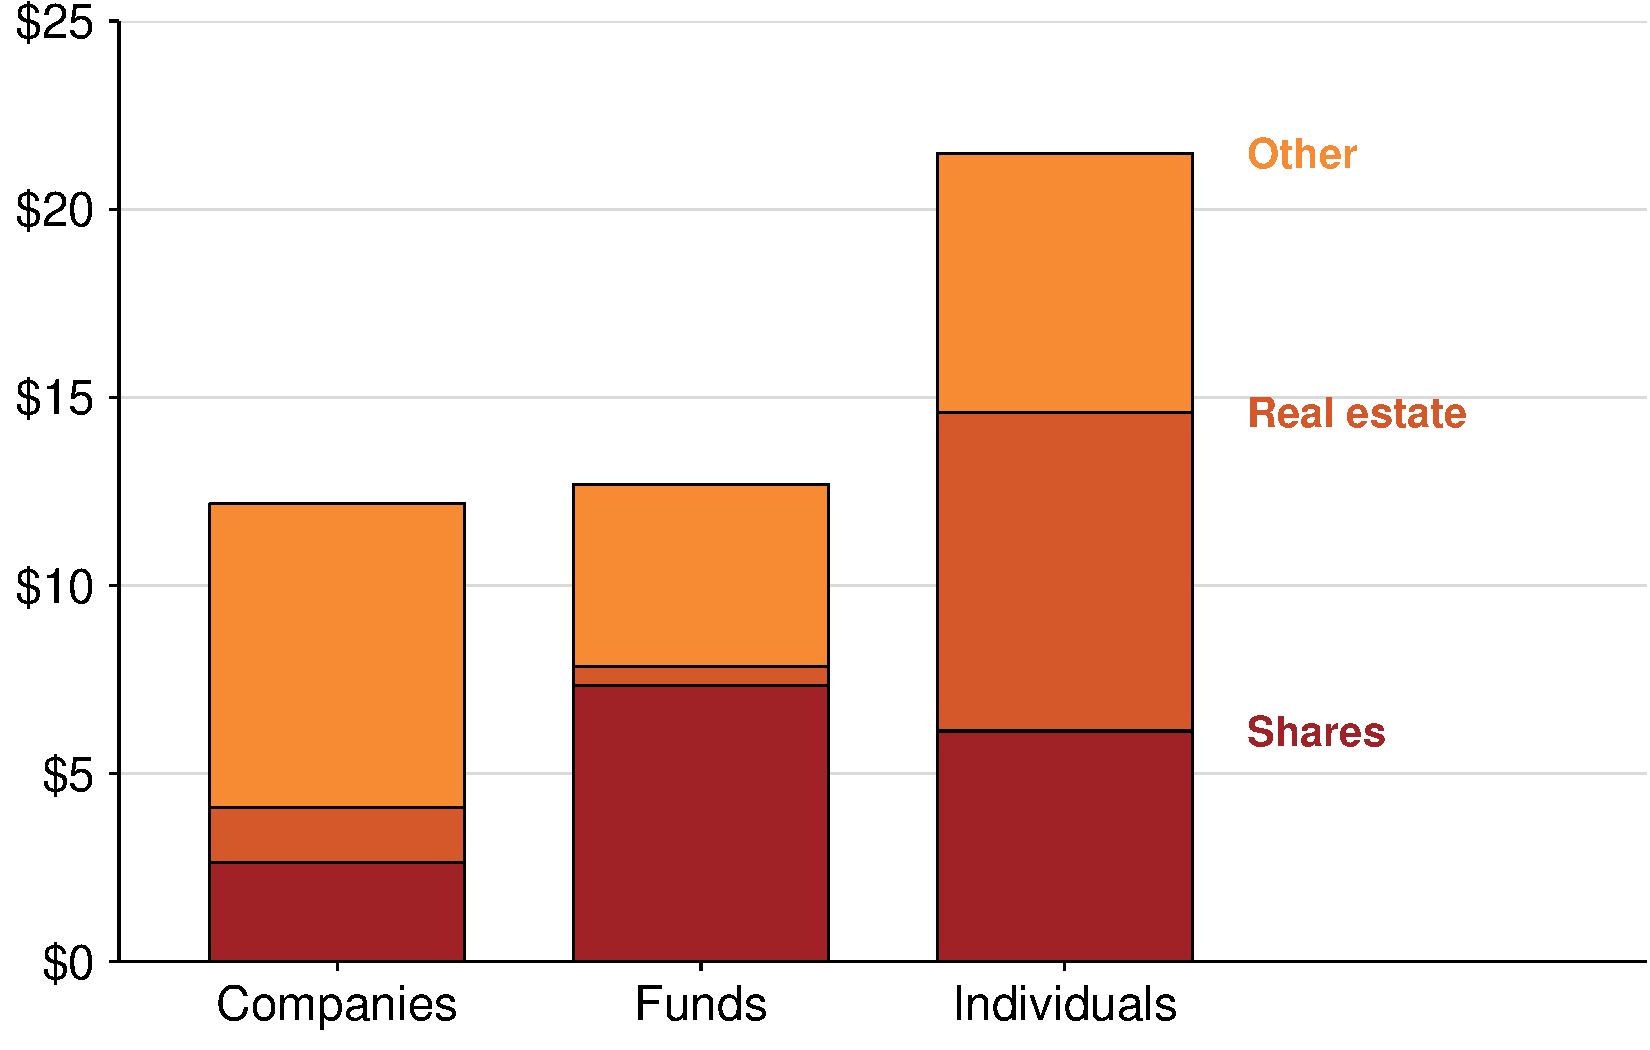
\includegraphics[width=\columnwidth]{figure/Majority_of_taxable_gains_are_earned_by_individuals-1}
\source{Molten combination of \textcite{ATOCapitalGainsByType}}
\end{figure}


\begin{smallbox}{A short history of capital gains tax changes}{box:short_history_CGT}
Before 1985 capital gains were untaxed in Australia. Taxes on capital gains were introduced to improve the integrity of the tax system, which was undermined by taxpayers recharacterising regular income as capital to avoid tax.\footcites{Evans2005}{Kenny2005}

Between 1985 and 1999, real capital gains (sale proceeds minus the original purchase price adjusted for inflation) were taxed at a taxpayer's marginal income tax rate. 

As recommended by the Ralph Review of Business Taxation, the Howard Government removed indexation adjustments so that tax was applied on nominal gains. To offset the removal of the indexation concession, capital gains tax was discounted by 50 per cent for individuals and 33 per cent for superannuation funds for assets held for more than a year. Capital gains of small unincorporated businesses, but not large businesses, are also discounted by 50 per cent. Small businesses also receive a range of other CGT concessions. When this regime was introduced, it was argued that it would stimulate capital markets and make the Australian regime more internationally competitive.\footcite[p.~14, 598]{BusinessTaxation1999} 

The tax concession is a crude way to adjust for the effects of inflation. It results in a lower tax bill compared to taxing real gains so long as asset values grow at least twice the rate of inflation. Given the strong real growth in asset prices, particularly residential property, since the discount was introduced governments have almost certainly lost revenue from the change.

\end{smallbox}
Before 1985, capital gains were not taxed in Australia. Since then, the tax treatment of capital gains has varied, but they are taxed at a lower rate than wage and salary income (\Vref{box:short_history_CGT}).  

Under the current rules, net capital gains are included as part of assessable income.\footnote{Capital losses can only be offset against capital gains, not ordinary income. But if taxpayers are unable to utilise their capital losses is a particular year, they are carried forward to future years \textcite{ATO2014a}.}  For individuals and small businesses, 50 per cent of their capital gains are excluded from income if they hold the asset for more than one year. This means the effective tax rate paid on these gains is half the rate for other forms of income. For superannuation funds, a third of their gains are excluded. Large corporations pay tax on all of their capital gains at the corporate tax rate of 30 per cent.

Capital gains have other less explicit tax advantages compared to recurrent income. Investors control when they realise gains. Consequently, they can reduce their tax by selling assets when their income is low, such as after retirement, so they are taxed at a lower marginal rate.\footnote{A common strategy for investors close to retirement is to shift capital assets into Self Managed Super Funds, and then sell them when they are aged over 60 and not liable for tax.}  For example, \textcite{Wood2010a} found that after adjusting for other factors, the probability of a landlord selling a property increases by over 20 percentage points once they retire.\footnote{The Age Pension asset test also encourages those moving into retirement to sell their assets. \textcite{Wood2010a}.}
Further, unlike other forms of income, capital gains are taxed on sale rather than as they accrue. This deferral of tax is akin to the government providing the investor with an interest free loan. (See \Vref{sec:ShouldCapitalGainsBeTaxedConsistently})

\section{Should capital gains be taxed consistently with other forms of income?}\label{sec:ShouldCapitalGainsBeTaxedConsistently}
Capital gains and other forms of savings income increase a person's spending power. It is arguable that all increases in spending power should be taxed consistently regardless of how they are earned (chapter 2)  or as the Canadian Carter report puts it ``a buck is a buck is a buck.''  Taxes on capital gains are highly progressive because most capital gains income is earned by the wealthy. Aligning tax rates for labour and capital gains also helps prevent tax arbitrage -- people converting labour income into capital gains to reduce their taxable incomes. 

On the other hand, increasing taxes on capital gains might reduce incentives to save and start new businesses. But personal income tax rates are not the most important determinants of these decisions. If nominal gains are taxed at the full marginal rate, we tax the inflation component of gains.  But with inflation rates low relative to investment returns, the 50 per cent discount overcompensates most investors. The discount also magnifies the tax advantages of capital gains over other investment income, such as bank deposits.

The other reason proffered for the discounted treatment of gains is to moderate the effect of `asset lock-in' whereby investors are deterred from selling assets that have accrued large gains. But the biggest causes of lock-in are investors waiting until retirement to realise gains or passing their assets (CGT free) to their beneficiaries. 

Most OECD countries offer some type of discount or concession for capital gains but it varies by investment type.\footnote{In some countries -- including Israel, Ireland, Norway, and Luxembourg -- property investments other than the family home are taxed as ordinary income. See \textcite{Harding2013} for a summary.}  But the hurdles to qualify for the most generous concessions can be stringent. Holding periods to receive maximum concession on investment property are ten years in Germany and Korea, 20 years in Slovenia, 30 years in France and 35 in Austria.\footcite{Harding2013} In New Zealand, where capital gains are notionally tax free, capital gains on property purchased with the intent to sell is taxed as ordinary income.\footcite[p.~25]{prebble2010tax} 
  
\subsubsection{Tax concessions for capital gains generate revenue leakage and favour the wealthy}
A lower tax rate for capital gains results in `revenue leakage' as taxpayers find ways to convert income into capital gains.\footcites{Evans2005}{Minas2013}  Protecting the income tax base is a key reason capital gains are taxed in most OECD countries\footcite{OECD2006b} and motivated the introduction of capital gains in Australia (see \Vref{box:short_history_CGT})

Traditionally this type of tax shelter has been the preserve of the wealthy. Executives paid via shares or stock options\footcite{Ingles2009}[pp.8-9] or corporate reorganisations of private corporations to convert dividend income into capital gain, for example.\footcite{Minas2013} But borrowing to finance investments with negative income flow but positive capital gains is another way in which wage income is effectively converted into capital gain for tax purposes. This comes about via the interaction of negative gearing with the capital gains tax provisions (\Cref{sec:negative_gearing_provides}). With more widespread availability of credit, and lower taxes on capital gains, this has become a far more popular tax minimisation strategy, increasing the cost of revenue leakage to the budget.

Lower taxes on capital gains also distort investment choices. They create an incentive for investors to choose assets more likely to generate income through capital gains rather than operating income.

\subsubsection{Tax concessions on gains favour the wealthy}
Tax concessions for capital gains favour wealthy taxpayers who receive most of the capital gains. Almost 80 per cent of capital gains are earned by those in the top 20 per cent of income earners (\Vref{fig:Nearly_eighty_per_cent_of_capital_gains_are_earned_by_those_}). Compared to low income earners, higher income earners are more likely to have additional income that can be invested.\footnote{The top 20 per cent of households by disposable income save on average 35 per cent of their disposable income. This compares to dissavings of 25 per cent for the lowest income quintile and savings rates of less than 10 per cent for the second and third quintiles.}


\begin{figure}
\Caption{Most capital gains are earned by those in the highest income decile although less when capital gains income is excluded}{Amount of net capital gains by income decile}{fig:Nearly_eighty_per_cent_of_capital_gains_are_earned_by_those_}
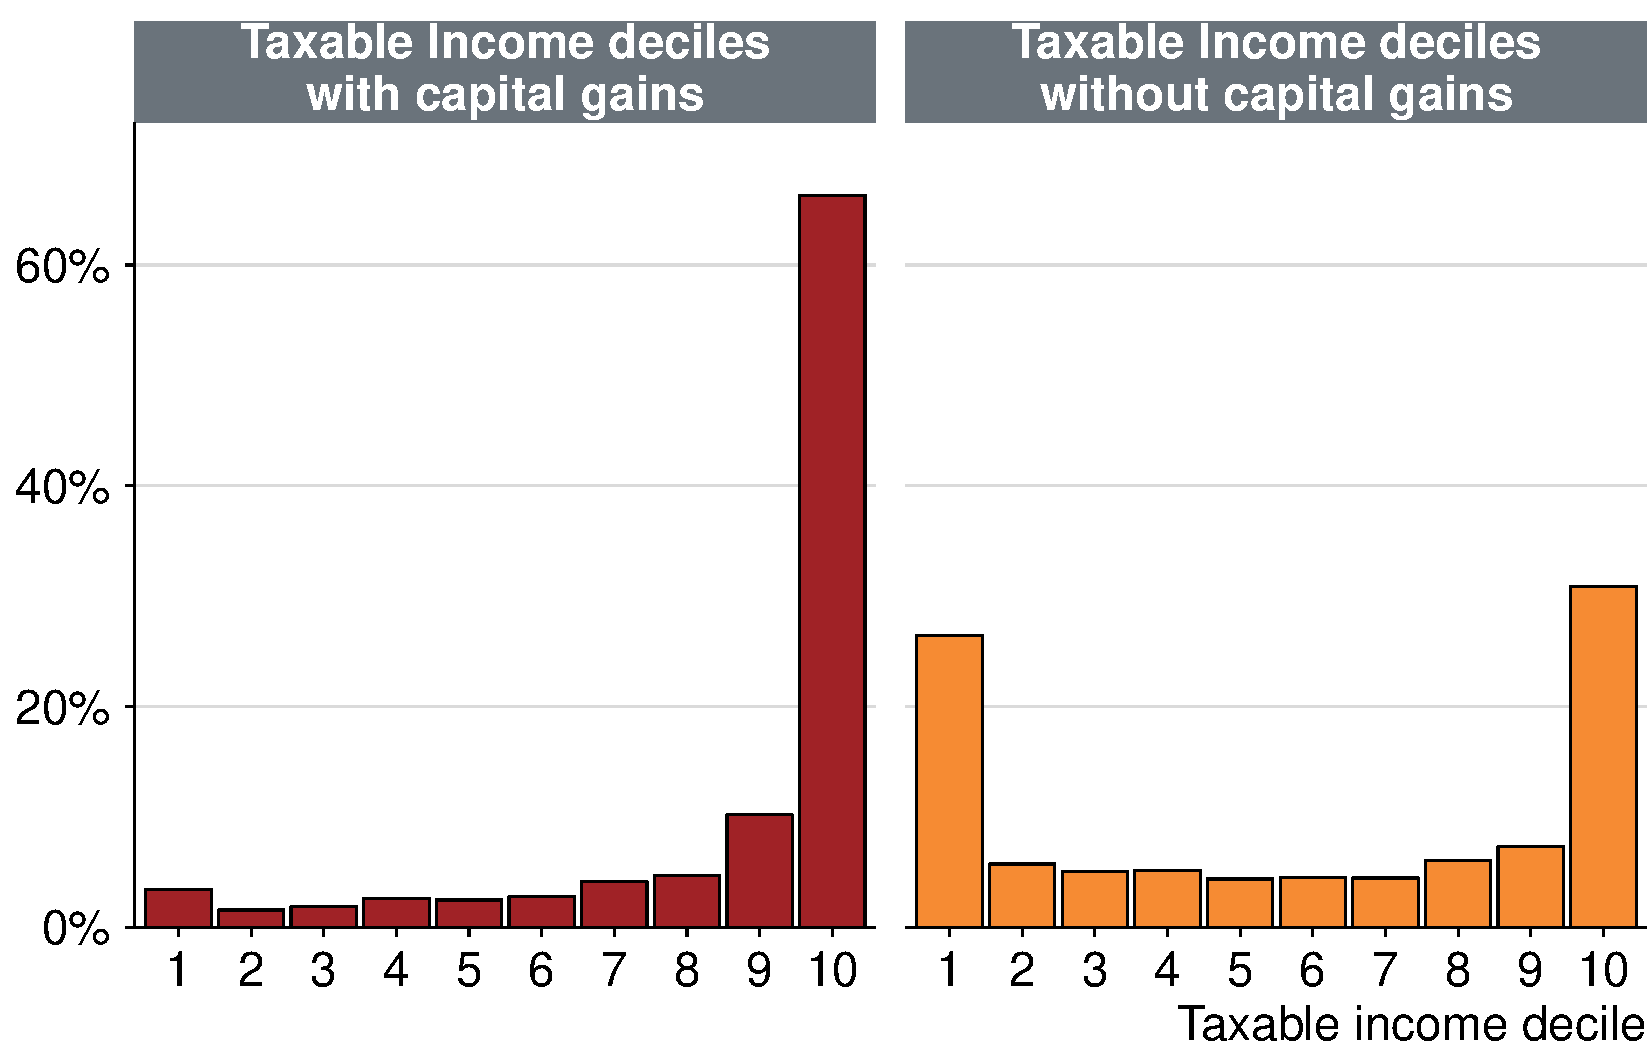
\includegraphics[width=\columnwidth]{figure/Nearly_eighty_per_cent_of_capital_gains_are_earned_by_those_-1}
\source{\gao\ \textcite{ATO2013i}}
\end{figure}
Some of this is accounted for by the `lumpy' nature of gains. This means that realising gains can push investors up the taxable income scale. When we control for this by removing gains from income, we see that more than 30 per cent of gains are still earned by those in the top ten per cent of (non-capital gains) income. 

A large fraction of gains are also earned by those would be in the bottom ten per cent of income earners but for their capital gains income (\Vref{fig:Nearly_eighty_per_cent_of_capital_gains_are_earned_by_those_}). As we show later, much of this is explained by the ``retirement realisation effect'' whereby people hold on to their assets until retirement so they can realise their gains when their taxable income is low. 


\subsubsection{The CGT discount overcompensates for inflation and is not consistent with the treatment of other investment income}
A lower tax rate for capital gains is sometimes justified on the basis that the effective tax rates on real returns can be high if nominal gains are taxed at marginal income tax rates.\footcite{Treasury2010} This is particularly true of investments with low real returns that are held for an extended period (\Vref{box:short_history_CGT}).

The tax concession is a crude way to adjust for the effects of inflation. In a world with constant tax scales, the 50 per cent discount results in a lower tax bill compared to taxing real gains so long as asset values grow at least twice the rate of inflation. In the current low inflation environment, the 50 per cent discount overcompensates most investors.\footnote{}

Making additional inflation adjustments for capital gains magnifies the tax advantages capital gains receive over other investment income. Ironically Australia's current system provides no adjustments for the least protection to bank deposits -- disproportionately held by the least well off -- and much more protection for other investments.\footnote{Over 90\%\ of those in the bottom decile have deposits, but less than 30\%\ have superannuation assets; and less than 20\%\ have equities or life insurance.}

Unlike other investment income, gains are taxed when an asset is sold, not when they accrue, which provides investors with an implicit interest-free loan on tax liabilities (\Vref{box:Tax_deferral_and_effective_tax_rates}).\footcites[See also:][p.~2]{Fane2004}[p.~12]{Ingles2009} Investors are also able to choose the time of the asset's disposal to minimise tax. 

\afterpage{%
\begin{bigbox*}{Capital gains enjoy tax-advantaged status over other forms of income}{box:Tax_deferral_and_effective_tax_rates}
Even without a discount, capital gains are taxed at a lower effective rate than other forms of investment income such as interest or dividends because the tax can be deferred until the asset is sold. This tax deferral is akin to an implicit interest free loan from the government. The tax benefits from this implicit loan increase the longer the asset is held. 

For example, consider a property that does not generate any recurrent income (rental payments just cover the annual expenses) but is expected to appreciate in value at 7 per cent a year. With no CGT discount, an investor in the top (47 per cent) marginal tax bracket is taxed at 23.5 per cent on the gains if they hold the property for a year. If the asset is held for 5 years the effective tax rate falls to 21.2 per cent. After 20 years it reduces to 14.6 per cent. 

In contrast, if the investor chooses a term deposit paying 7 per cent a year and they reinvest the after-tax income each year, their effective tax rate is 47 cents a year, regardless of the holding period for the asset. (See \Vref{fig:Real_effective_marginal_tax_rates_are_lower})

The capital gains tax discount magnifies the tax advantaged status of capital gains. 
\eject

\captionoffigurewithunits{Real effective marginal tax rates are lower for capital gains than income, especially after the capital gains tax discount}{Real effective marginal tax rate}\label{fig:Real_effective_marginal_tax_rates_are_lower}
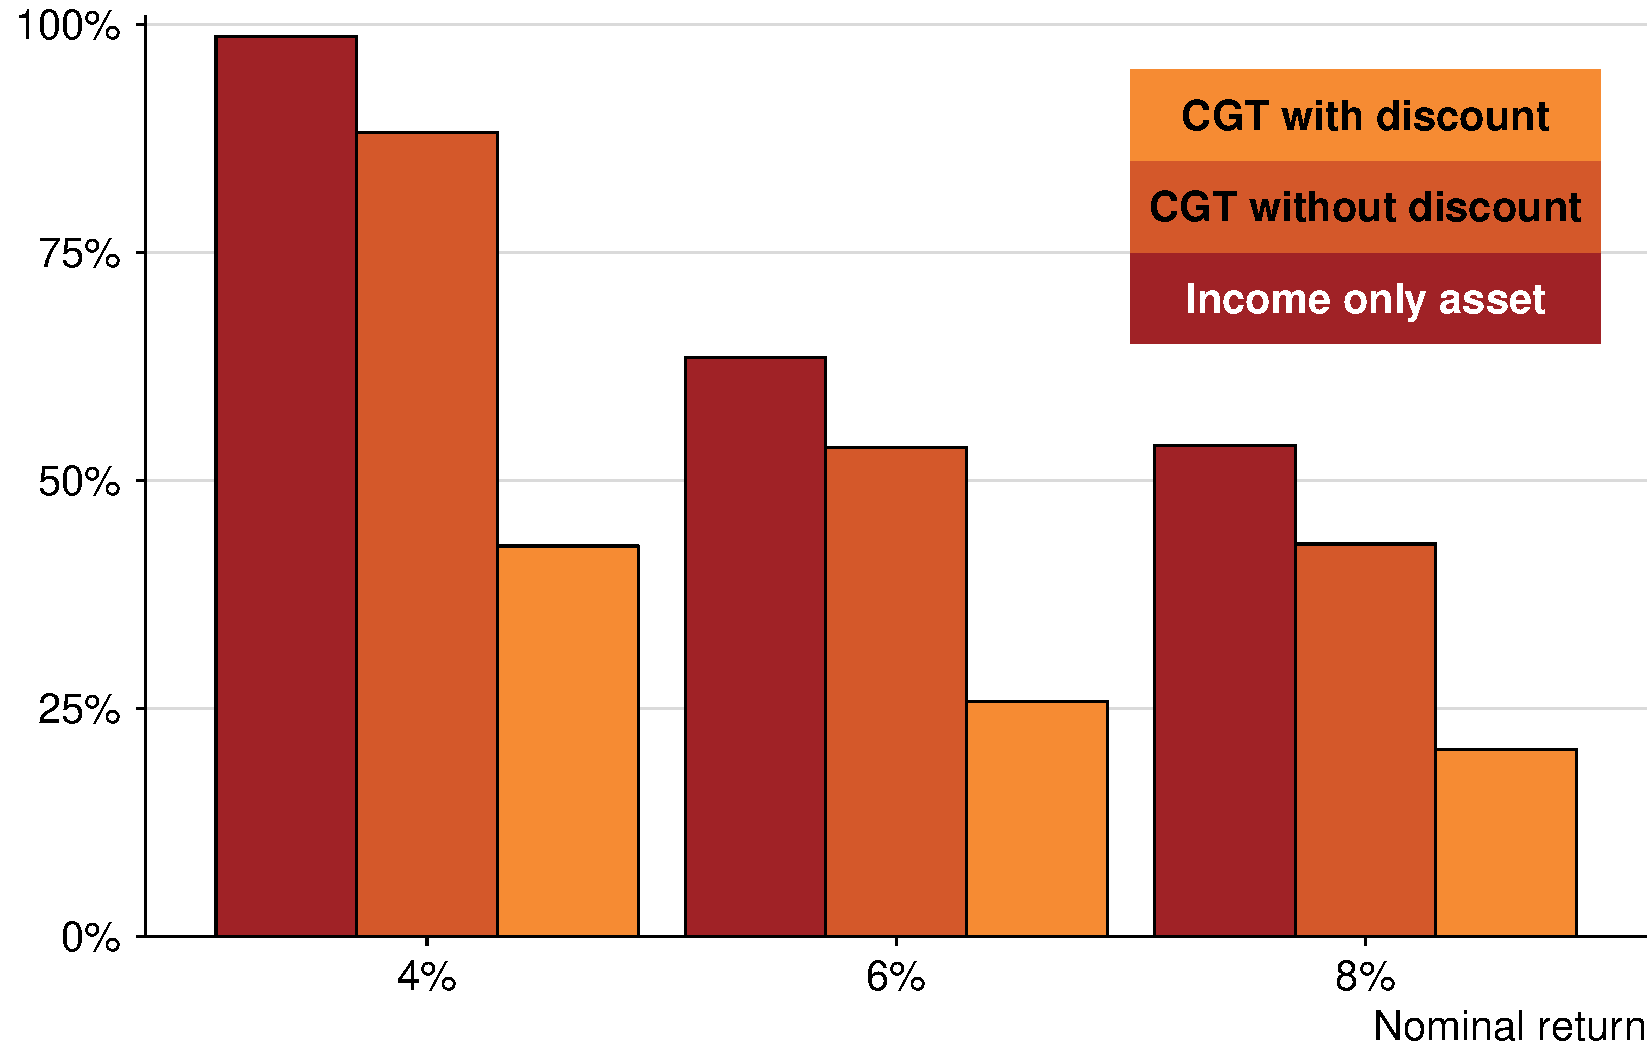
\includegraphics[width=\columnwidth]{figure/Real_effective_marginal_tax_rates_are_lower-1}
\source{Grattan analysis}
\end{bigbox*}
}

\subsubsection{Taxing capital gains without a discount will not substantially distort economic decisions}
Taxing capital gains at the full marginal rate could deter entrepreneurship and risk taking by reducing the returns to selling a successful business.\footnote{If capital gains were taxed on an accrual basis and capital losses were fully deductible against all assets, then taxing gains in full would be neutral with respect to risk. However, since losses are only deductible against gains this increases the risk that investors will make a loss they are not able to deduct. It is not clear whether deferral of taxes on gains until realisation, itself a significant tax advantage (section x.1), is itself enough to compensate investors for this risk. \textcite[p.~8]{Burman2009};  \textcite[p.~130]{Commission2004}}  But this effect may not be large. There are other factors that drive entrepreneurship and risk taking behaviour that are far more significant than the tax on any gains ultimately made.\footcite[p.~75]{Burman1999}   Further, other exceptions already in place limit the effects of capital gains tax when assets or businesses are sold.\footnote{Capital gains tax exemptions are available for the sale of active assets by small business up to a lifetime limit of \$500,000 provided the gains are paid into a complying super fund. There are also exemptions for people over 55 that are retiring and selling business asset held for more than 15 years. Small business also receive rollover relief allowing them to defer all or part of a capital gain for two years or longer on the sale of active assets, provided they acquire a replacement asset or you incur expenditure on making capital improvements to an existing asset. \textcite{ATO2014e}} In any case, gains received from the sale of business are a small proportion of total gains from individuals: most are from property and share-market investments (\Vref{fig:Majority_of_taxable_gains_are_earned_by_individuals})

While mixed, empirical evidence suggests that aggregate savings may not be particularly responsive to tax rates, particularly for high income earners. For example, \textcite{Engen1996} finds that tax breaks for saving influence the choice of savings vehicle but do not increase overall household savings much. And the OECD finds that tax breaks for saving are generally ineffective for high income earners because this group are likely to save anyway.\footcite{OECD2007}  \textcite{chetty2013subsidies} show that reduced subsidies for retirement savings for high income earners lead to almost no reduction in overall savings efforts.\footnote{\textcite{chetty2013subsidies} ) is a particularly compelling study because of the strength of the data (41 million observations on savings for people from Denmark). But it is also consistent with the thrust of the literature on the effect of tax incentives for retirement savings. While findings vary across studies, a summary by \textcite{Antolin} suggests tax incentives increase savings mostly by reallocation from other savings vehicles. }

This suggests that larger distortions arise from the different tax treatment of different forms of savings than from the weight of taxes on capital in general.\footcite[p.~16]{Ingles2009} 

\subsubsection{People may hold assets longer, but many already wait until retirement}
The other economic cost of higher taxes on capital gains is greater asset lock-in. 

Because taxes are only paid when gains are realised, investors are encouraged to hold on to assets with large accumulated gains.\footcite[p.~69]{Burman2009} In effect, the investor seeks to maintain the implicit interest free loan on accrued gains. Crystallising a capital gain is only worthwhile if an investor can achieve a materially higher return (\Vref{box:CGT_asset_lockin}).\footcite[p.~12]{Ingles2009}

Lock-in can discourage investors from moving their money to the investments with the highest pre-tax returns, so assets do not always go to their highest value use.\footcite{Lindsey1987} Lock-in effects are most significant from a whole of economy perspective, if they constrain financing of profitable investments.\footcites{OECD2006b}{Johnson2008}  Australia's open capital markets and generous capital gains tax regime for non-residents, reduce the danger that worthwhile projects will not get access to capital because of lock-in.\footnote{Non-resident investors in Australian shares are generally not subject to Australia capital gains tax (see: \emph{Income Tax Assessment Act 1936, s. 136-25}} 

The more fundamental cause of lock-in is the ``retirement realisation effect'' -- the tendency for investors to wait until retirement when their taxable incomes are low before realising gains.
 \textcite{Wood2010a} found that after adjusting for other factors, the probability of a landlord selling a property increases by over 20 percentage points once they retire.
 
\begin{smallbox}{Capital gains tax and asset lock in}{box:CGT_asset_lockin}
Suppose Hayley, an investor in the top tax bracket purchases a house for \$700,000 and holds it for 10 years. During that time the market price of the house increases to \$1 million. She makes a net rental return of 5 per cent a year, giving her a \$50,000 income stream. 

If she were to sell the house she would crystallise the \$300,000 in gains, paying tax on 50 per cent of the gains at her marginal tax rate of 49 per cent (\$73,500). This would leave her with around \$926,500 from the sale: \$226,500 in net gains and her initial investment of \$700,000. In order to better her income of \$50,000 and make the sale worthwhile, she needs to find an investment (with the same opportunity for capital gains) that pays net returns of more than 5.4 per cent a year.

If capital gains were taxed in full, rather than at the current 50 per cent discount, her hurdle rate for the new investment would be 5.9 per cent. 
\end{smallbox}

We can see the retirement realisation effect in the patterns of capital gains realisation by age. Those over 50 have much higher average realisation of gains, regardless of income level.


\begin{figure}
\Caption{Taxpayers wait till retirement to realize capital gains.}{Incidence of capital gain events in 2012-13, by age and income}{fig:Prob_of_CGevent_by_age_income}
\includegraphics[width=\columnwidth]{figure/Prob_of_CGevent_by_age_income-1}
\source{\gao\ \textcite{ATO2013i}}
\end{figure}
And many of those 50 to 64 -- the peak retirement years\footnote{The average age at retirement from the labour force for people aged 45 years and over in 2012-13 was 53.8 years (58.5 years for men and 50.0 years for women). \textcite{ABS2013}} -- realise sizeable gains when their other taxable income is low, suggesting they are waiting until retirement. Indeed, almost 60 per cent of the capital gains in this age group are earned by the 24 per cent of people without wage and salary income. 

The other group that realise a lot of capital gains are high income older people. Many of these will be people moving assets inside their Self Managed Super Fund in anticipation of retirement.\footnote{}

The other important cause of lock-in is the fact that capital gains are disregarded on death. Passing assets to a beneficiary is not regarded as an ``event'' that triggers a capital gains tax liability. So by passing on assets to heirs, capital gains taxes can de deferred indefinitely. 

Ultimately, the best way to reduce asset lock-in is to tax gains on an accruals basis, with interest charges on the deferred tax.\footcite[pp.~11-14]{Burman2009} This would remove the incentive to hold on to gains to reduce the tax burden. 

To date, annual asset revaluations have been considered impractical and beset with administrative difficulties.\footcites{OECD2006a}{Commission2004} But such valuations can be done easily for shares and to a lesser extent property (which is already revalued in most states every one or two years for the purposes of levying council rates (chapter 5)).\footcites{Burman2009}[p.~12]{Ingles2009} The Henry review flagged that such an accruals approach to capital gains becomes more feasible as technology improves.\footcite[p.~64]{Treasury2010} 


\section{Negative gearing benefit provides generous tax treatment for investors}\label{sec:negative_gearing_provides}
Negative gearing allows taxpayers to subtract the losses they make on investments (including mortgage interest payments) from their taxable income including wages. 

The ability to offset losses against other income is part of the normal operation of the Australian tax system, and applies to a wide range of investments and business activities. If losses were not deductible, they would be treated asymmetrically to gains (which are taxed) and investments in risky assets would be less attractive. Deductibility of interest payments in theory maintains tax neutrality for investors choosing between lending and equity financing.\footcite{Fane2004}  


But the issue for negatively geared property or shares is that the loss being deducted is illusory. Investors are only willing to make an income loss over a number of years because the value of the asset is growing. But the gains in property value are not counted as income until the asset is sold (section 1.2). It is the combination of unlimited deductions of "losses" against wage income while only being taxed on half the gains upon realisation that makes negative gearing an attractive strategy.\footcite[pages~5,13]{ACOSS} 

This comes at both a cost to the budget and potentially negative impacts in investment markets, particularly housing markets, where the tax treatment has encouraged speculative activity. 

\subsection{Negative gearing is growing in popularity, mainly for housing investment}
There has been a boom in negatively geared residential property investments over the last two decades. Other than a temporary dip following the global financial crisis, both the number of taxpayers making losses on residential property investment and the average loss made has increased steadily (\Vref{fig:Negative_gearing_real_over_time})




\begin{figure}[t]
\Caption{The introduction of the capital gains discount, but not the introduction of negative gearing, led a large fall in rental profits.}{Total net rent, billions (2013-14~dollars)}{fig:Net_rent_over_time}
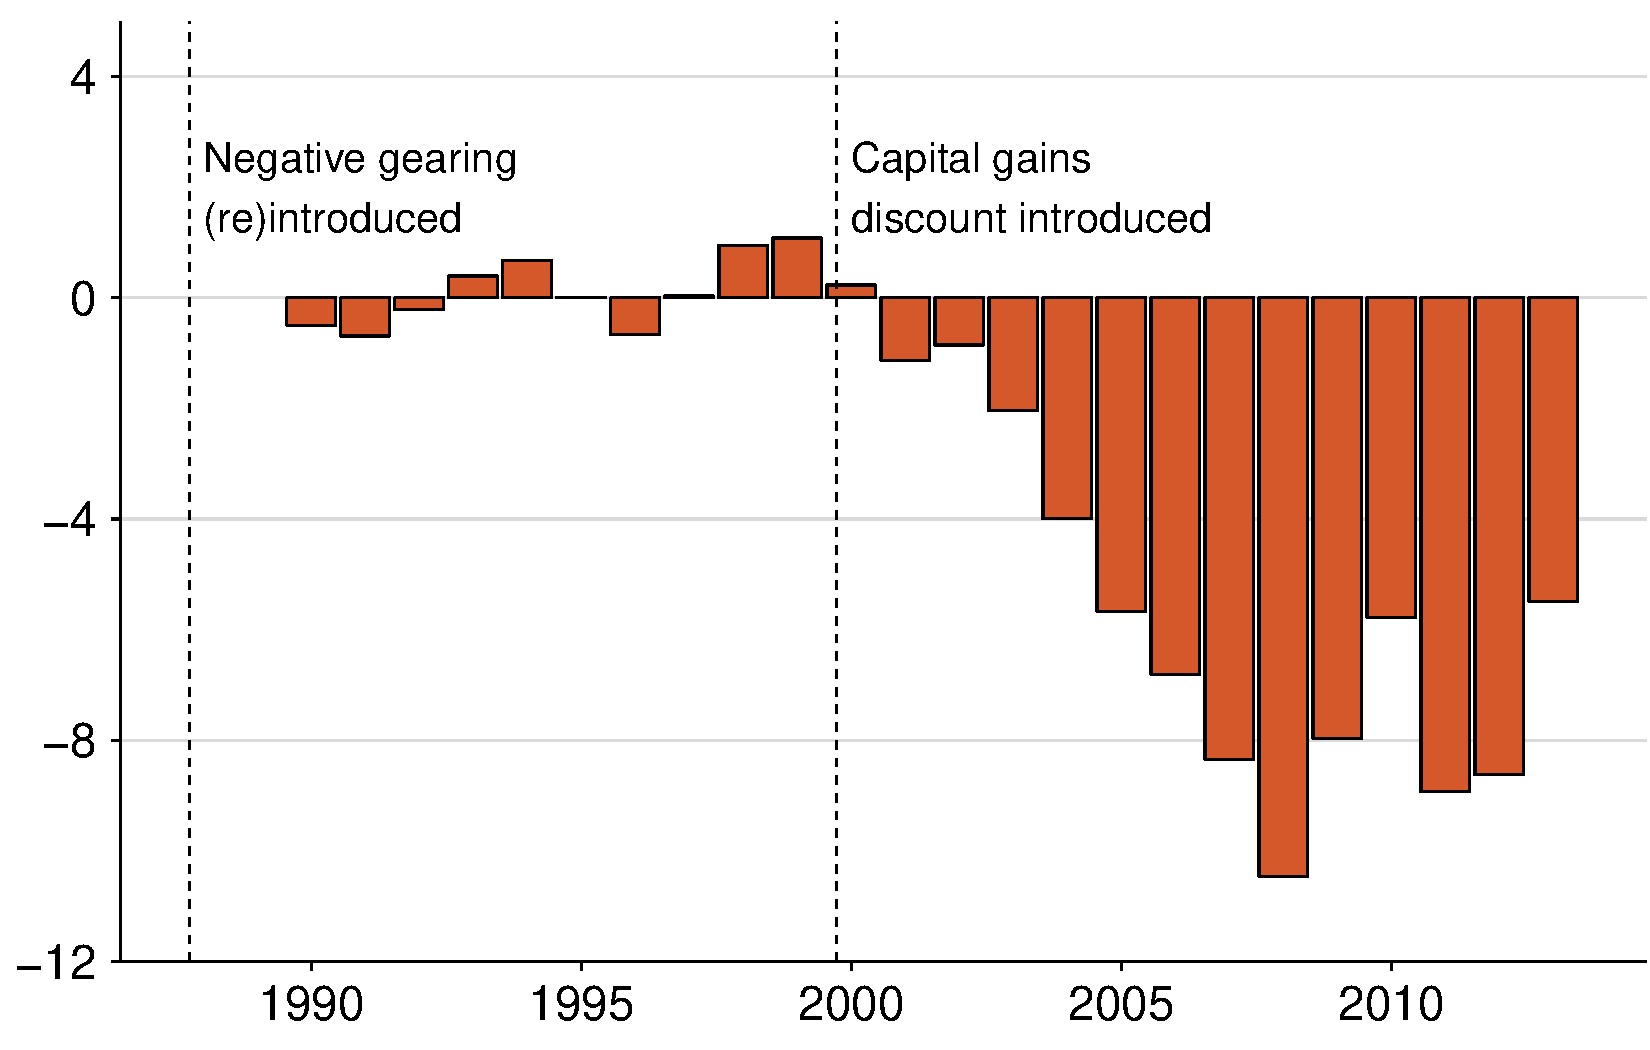
\includegraphics[width=\columnwidth]{figure/Net_rent_over_time-1}
\notes{Net rent as marked by taxpayer upon lodgement of tax return}

\source{ATO taxstats 1979-2013 (data not available pre-1989)}
\end{figure}

\begin{knitrout}
\definecolor{shadecolor}{rgb}{0.969, 0.969, 0.969}\color{fgcolor}\begin{kframe}
\begin{verbatim}
## Response [http://data.gov.au/dataset/e29ef9ca-0d1a-47ec-9e9b-14a79a941511/resource/5bfb5001-2d3c-46cb-a76d-1b86b6913ac3/download/taxstats2013company1selecteditemsforincomeyears197980to201213.xlsx]
##   Date: 2015-07-05 13:13
##   Status: 200
##   Content-Type: application/vnd.openxmlformats-officedocument.spreadsheetml.sheet
##   Size: 116 kB
## <ON DISK>  taxcompanies_time_series1979-2013.xlsx
\end{verbatim}
\end{kframe}
\end{knitrout}


\begin{figure}[t]
\Caption{Did companies divest of assets yielding negative returns for individuals to lap up, after the discount was introduced}{Net rent (companies), \$~billions, (2013-14 dollars)}{fig:Net_rent_over_time_companies}
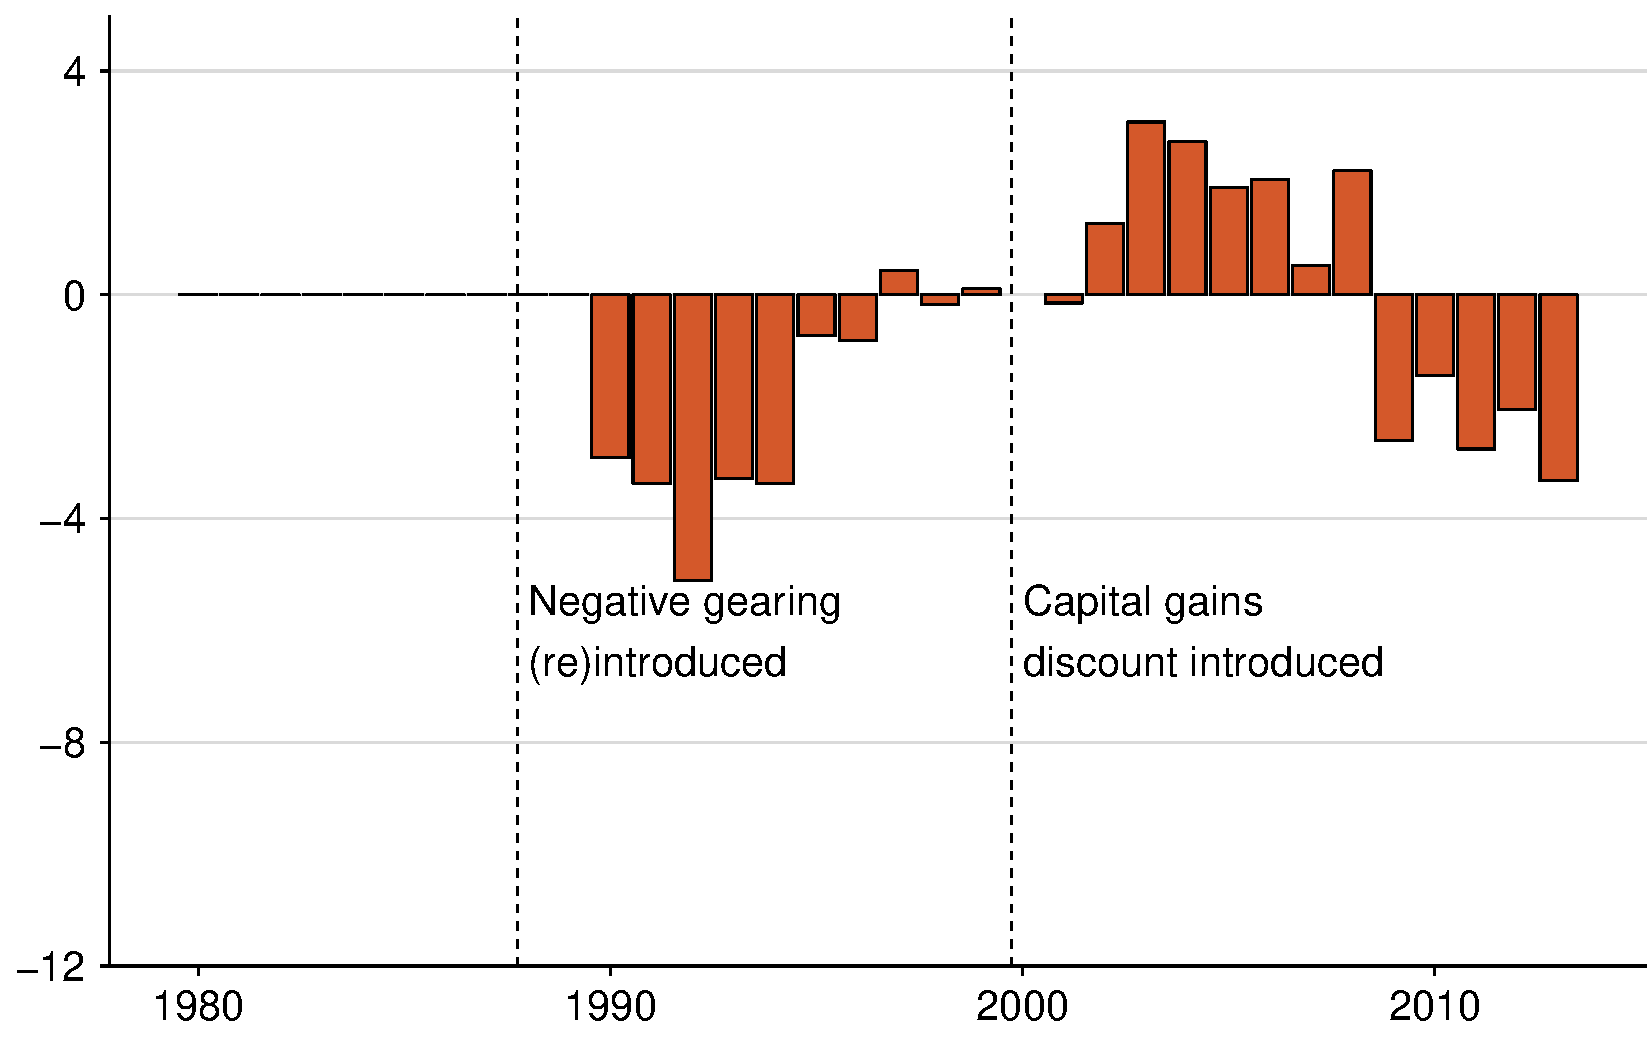
\includegraphics[width=\columnwidth]{figure/Net_rent_over_time_companies-1}
\source{Simple calculation of \url{http://data.gov.au/dataset/e29ef9ca-0d1a-47ec-9e9b-14a79a941511/resource/5bfb5001-2d3c-46cb-a76d-1b86b6913ac3/download/taxstats2013company1selecteditemsforincomeyears197980to201213.xlsx}}
\end{figure}



\begin{figure}
\Caption{More people are negatively gearing and the losses are growing even faster}{Number of people negatively gearing and real amount negatively geared (in 2012-13 dollars). First year = 1.}{fig:Negative_gearing_real_over_time}
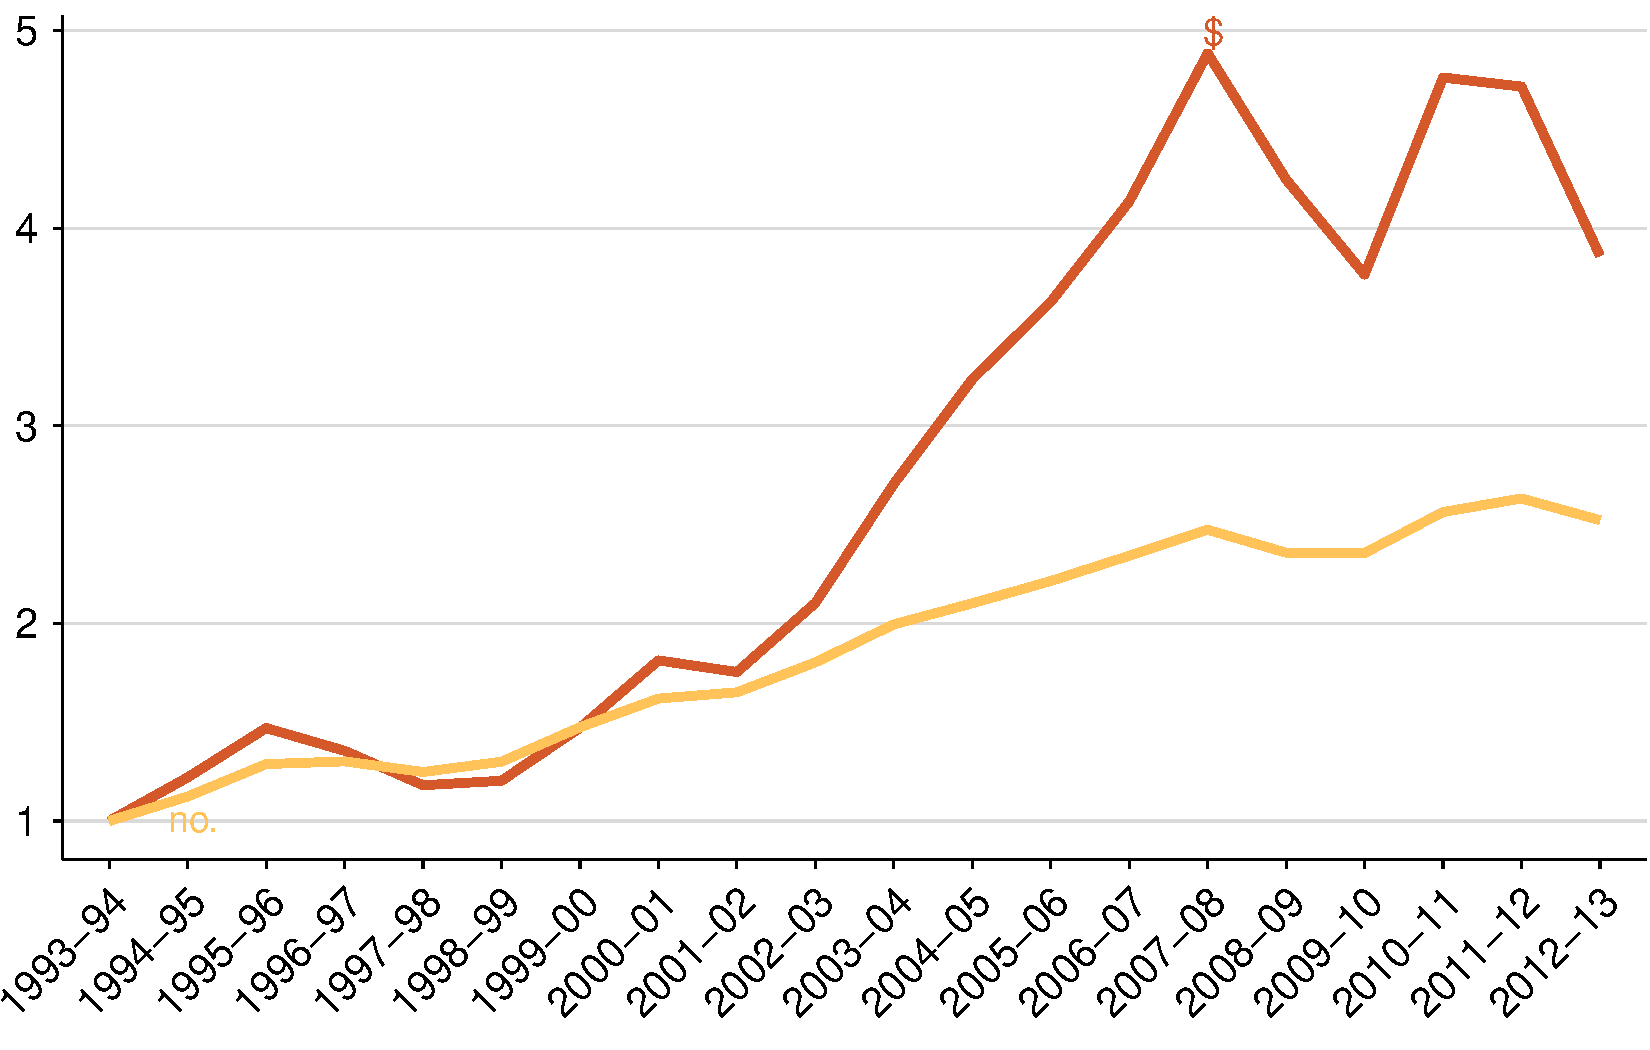
\includegraphics[width=\columnwidth]{figure/Negative_gearing_real_over_time-1}
\notes{Amount deflated by CPI. Other indices may be more useful.}

\source{\gao\ \url{https://data.gov.au/dataset/e29ef9ca-0d1a-47ec-9e9b-14a79a941511/resource/233cbf28-6fda-4e53-bbe9-3a37a65fb742/download/taxstats2013individual01selecteditemsbyyear.xlsx}}
\end{figure}
The average property investor is making a loss of more than \$5000 annually. The majority of the loss is mortgage interest payments. (\Vref{fig:Interest_makes_up_the_bulk_of_rental_deductions})


\begin{figure}
\Caption{Interest makes up the bulk of rental deductions}{Rent and deductions for residential property investors, billions of dollars (2012-13)}{fig:Interest_makes_up_the_bulk_of_rental_deductions}
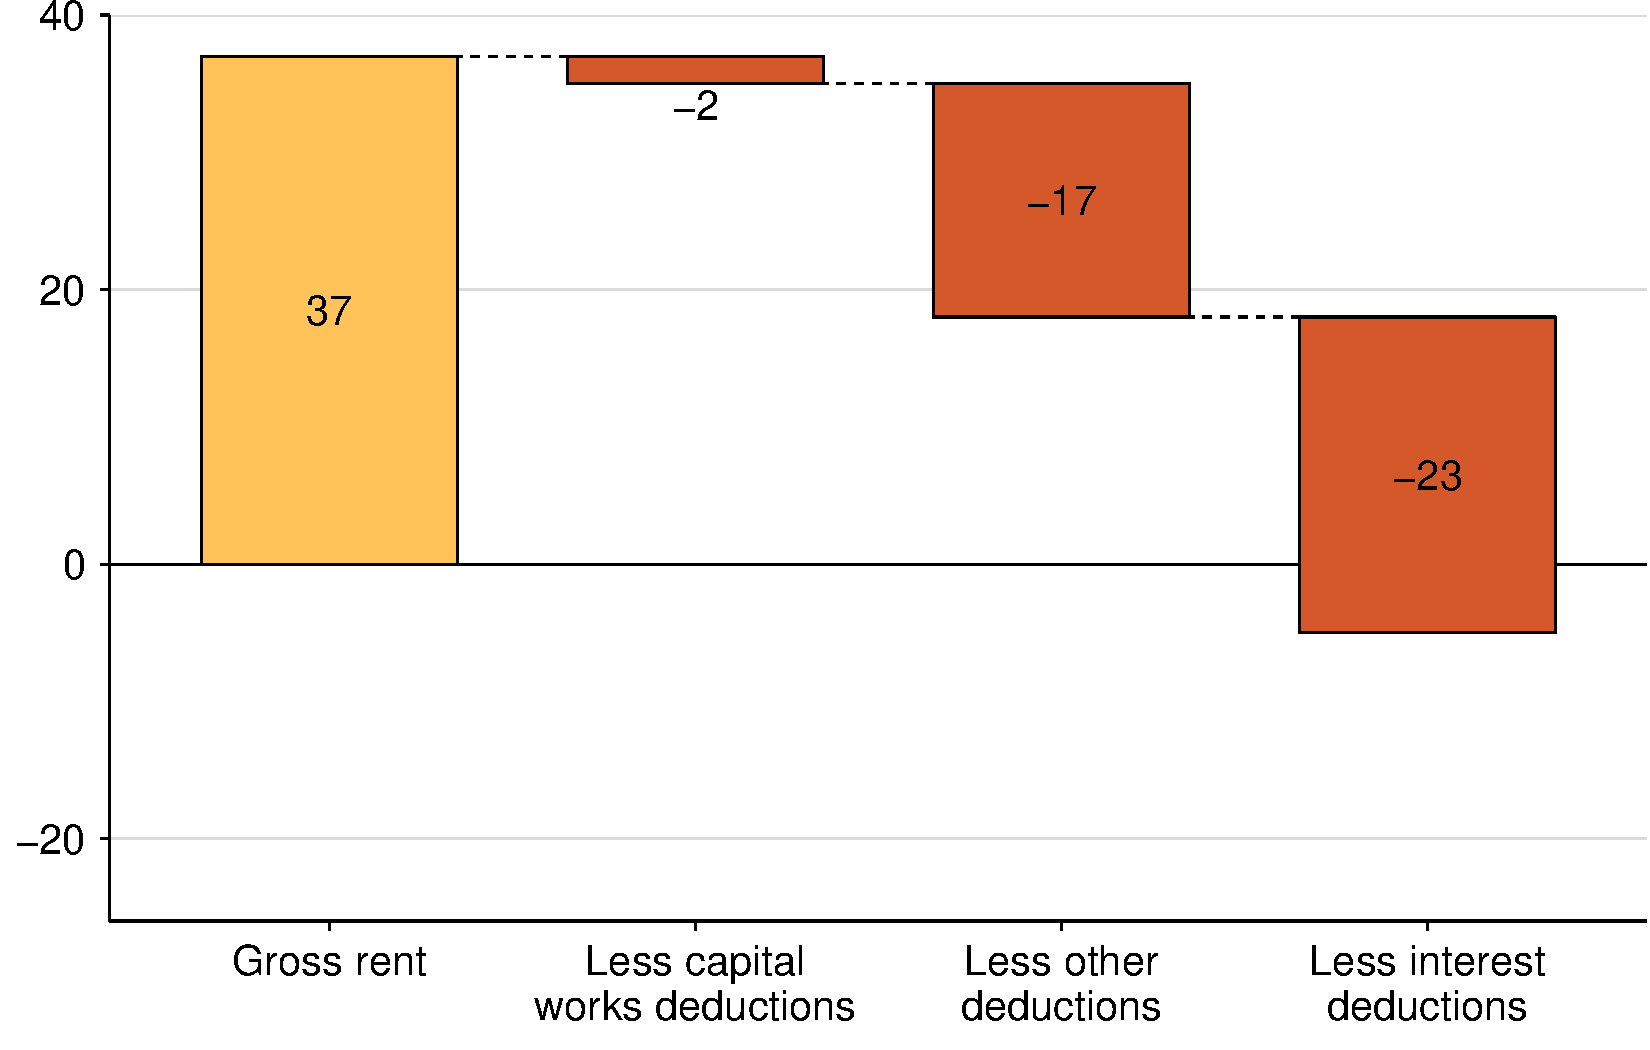
\includegraphics[width=\columnwidth]{figure/Interest_makes_up_the_bulk_of_rental_deductions-1}
\notes{}

\source{Grattan analysis of \textcite{ATO2013i}.}
\end{figure}

Negative gearing is used much less for investments outside of housing. Even at the height of the share market boom, only about 10 per cent of investments outside of superannuation were funded by borrowing -- and many of them were positively geared;\footcite{Daley2007}  since then margin lending has reduced by around 70 per cent from its peak in 2007.\footcite{RBA2015a}
\subsection{Interaction with capital gains tax discount encourages leveraged and speculative investment activity}
Taxes on capital gains are discounted by 50 per cent and only paid when the asset is sold. But negative gearing arrangements allows investors to deduct ``losses'' -- investment expenses  (including interest costs) in excess of rental income from wage income that would otherwise be taxed at the full marginal rate.\footnote{In reality, the assets are generally not making a loss because they accruing a capital gain. It is simply that this gain is not taxed until realisation. See: \textcite{ACOSS}[pp.~12-13.]}

This makes it more attractive to invest in assets that offer low returns on the expectation of future capital growth. This has played a role in investors being prepared to accept rental yields that are lower than those seen in other countries. As \textcite[p.~42]{RBA2014} notes:

\begin{quote}
\dots in most countries the earning of rental income is seen as the most important reason for investing in rental properties. \dots\ This seems to stand in contrast to the situation in Australia where properties are commonly marketed on the presumption that they do not earn positive taxable income for a considerable period.
\end{quote}

The asymmetry between the tax treatment of gains and losses also makes debt financing of investment more attractive. The Henry tax review estimated that for a high income taxpayer investing in a rental property, effective marginal tax rates are negative for a 70 per cent geared property, but almost 50 per cent if the property is owned outright.\footnote{For a tax payer on 46.5 per cent marginal rate (the top tax rate at the time), 6 per cent nominal return, 2.5 per cent inflation, 50 per cent return attributed to capital gains and 50 per cent to rental income. Rental property held for 7~years. \textcite[p.~74]{Treasury2010}}  It described the asymmetry between gains and losses as ``among the greatest tax induced biases to the savings choices of households''.\footcite[p.~69]{Treasury2010}  This runs contrary to the rationale for allowing the deductibility of losses -- to maintain tax neutrality of debt and equity financing. 

Borrowing to finance an investment with low yields but high potential capital appreciation allows an investor to reduce and defer their tax by effectively converting salary income into capital gains. 

The effect is to incentivise leveraged and speculative investments, particularly for property.\footcite[p.~17]{Inquiry2014} Investors have responded to these incentives. Before the capital gains tax discount was introduced in 1999, there were 1.3 million landlords making an aggregate taxable profit of \$0.7~billion. By 2012-13, there were 2 million landlords making collective losses of \$5.5 billion.\footcites{Eslake2013}{ATO2015} Over this same period, the proportion of property investors making losses on their investment increased from around 50 per cent to 65 per cent.\footcite{ATO2014e} 

The average level of gearing for property investors is increasing. Even though interest rates are falling, interest deductions as a proportion of rents increased from 45.6 per cent of gross rental payments in 1997-98 to 71.1 per cent in 2011-12.\footcite[p.~65]{Treasury2015}

The favourable tax treatment for investors drives up house prices because it increases the after-tax returns to housing investors.\footnote{FOr example, \textcite{Commission2004} found that these tax settings had added to the housing price boom by encouraging investors to reduce current income in favour of longer term gains.} This helps existing home-owners but accelerates falling rates of home ownership among younger age groups.

\subsection{Reducing tax on wage income is particularly attractive}
Using negative gearing to reduce and defer tax is a particularly attractive strategy for those with high wage incomes. Of course, negative gearing only makes sense if the expected capital gains (and any positive income) exceed the income losses over the time the asset is held. But for some investors, reducing taxes on their wages has become one of the primary goals. Investment advisors frequently warn investors against placing too much emphasis on tax breaks and not enough on the financial returns to the investment.\footcite[See for example:]{Brown2012}

The attractiveness of using investment losses to reduce taxes on wage income is evident in the age profile of those negatively gearing property. (\Vref{fig:Age_negative_gearing_investments}) Investing in loss making properties is popular amongst those of working age, but far less prevalent amongst over 60s who are unlikely to benefit from the tax write-offs. Over 60 per cent of those under 60 with investment properties make rental losses compared to less than 40 per cent over 60. 

\begin{knitrout}
\definecolor{shadecolor}{rgb}{0.969, 0.969, 0.969}\color{fgcolor}\begin{kframe}


{\ttfamily\noindent\bfseries\color{errorcolor}{\#\# Error in fread("{}2013\_sample\_file.csv"{}): File is empty: C:\textbackslash{}Users\textbackslash{}HPARSO\textasciitilde{}1\textbackslash{}AppData\textbackslash{}Local\textbackslash{}Temp\textbackslash{}Rtmpq8HsgE\textbackslash{}file3fec18e6412f}}\end{kframe}
\end{knitrout}
\begin{figure}
\Caption{More people negatively gear investments in their peak earning years}{Negative gearing status, percentage within each age group.}{fig:Age_negative_gearing_investments}
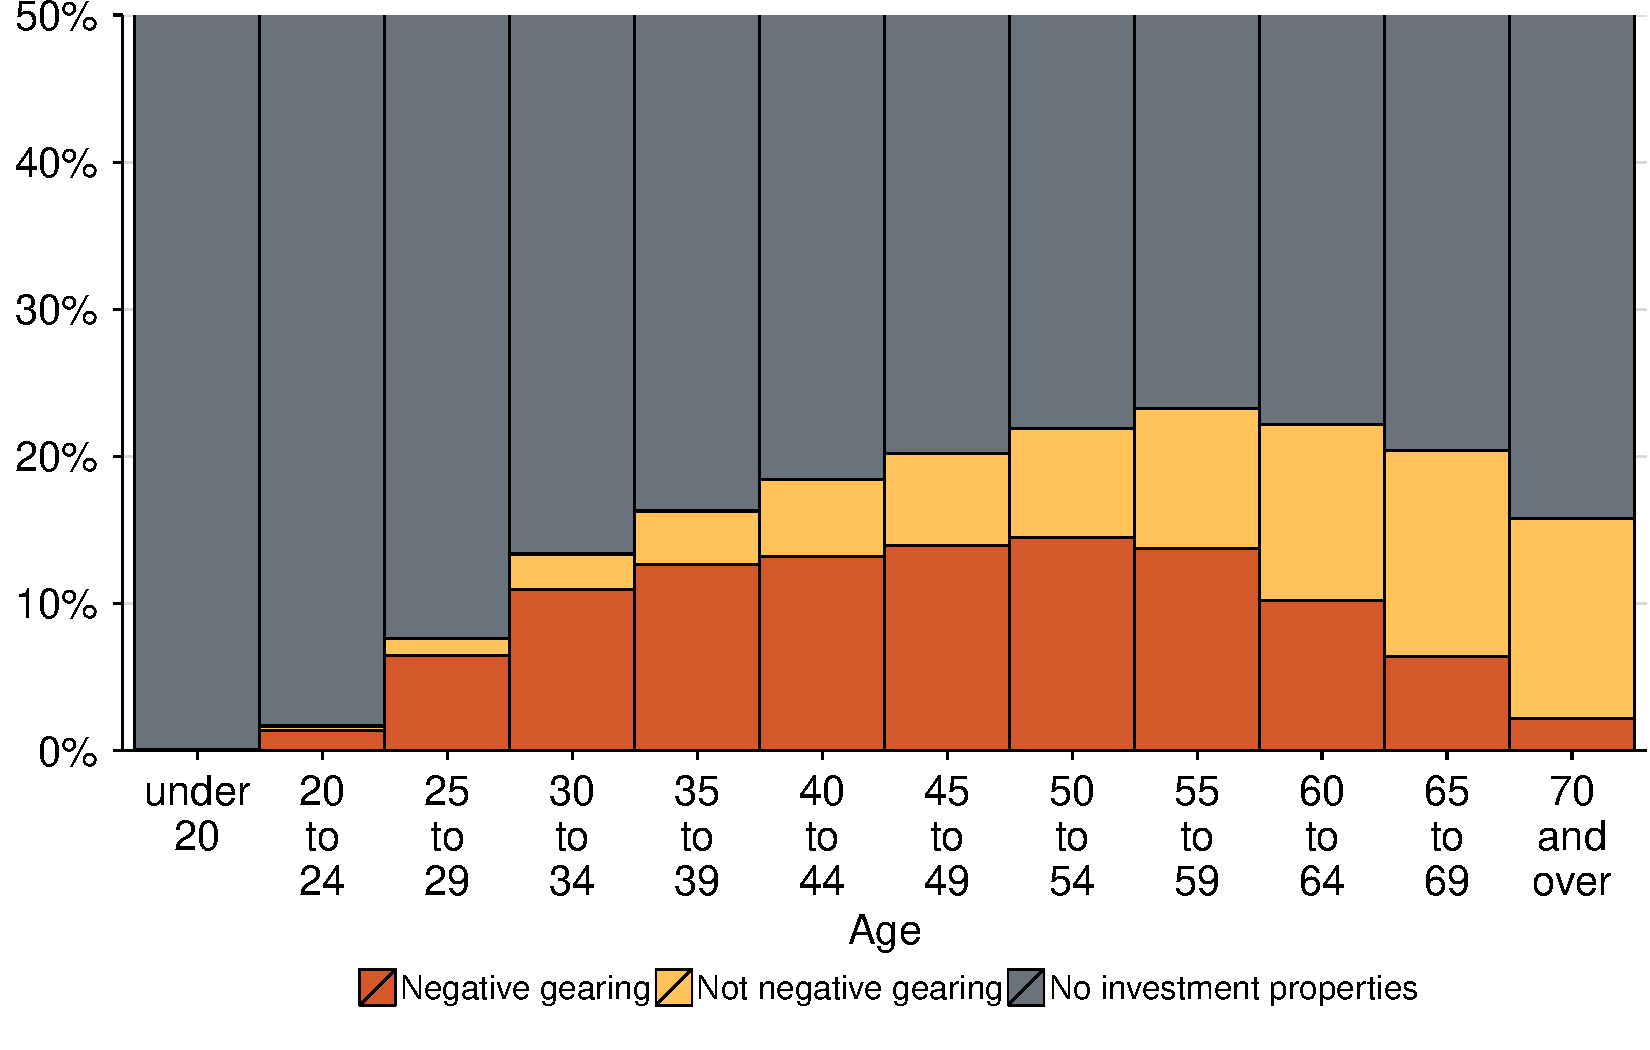
\includegraphics[width=\columnwidth]{figure/Age_negative_gearing_investments-1}
\notes{The top 50\%\ of the chart is not shown -- it would be grey all the way to 100\%. ``No investment properties'' means gross rental income is zero.}

\source{\gao\ \textcite{ATO2013i}}
\end{figure}

Most other advanced economies provide a less generous treatment for rental losses. The Unites States only allows losses to be written off against other forms of ``passive'' income. The UK and many European countries only allow deductions against the same class of income, so for example, losses on investment property can only be used to reduce tax on income or capital gains from other investment properties. Others such as the Netherlands do not allow deductibility of losses from investment housing.\footnote{Summaries of international regimes can be found in \textcite[p.~43]{RBA2014} \textcite[p.~86]{Commission2004}, \textcite[pp.~92-95]{ODonnell2005}}% #820}. } 

\subsection{Negative gearing mainly benefits middle and high income earners}
Like most tax concessions on investment, tax benefits from negative gearing are biased to the wealthy. The increase in after-tax return as a result of the current negative gearing/capital gains interaction is larger for individuals on higher marginal tax rates, all else being equal.\footcite{Inquiry2014}   

The top 10 per cent of income earners receive more than one third of rental deductions. (See \Vref{fig:Effect_of_Deductions}.) If we look at tax deciles before rental property losses are deducted -- correcting for the fact that many better off taxpayers use rental losses to reduce their taxable income -- the top ten per cent of income earners receive almost fifty per cent of the tax benefits of negative gearing.\footnote{\textcite{RBA2015} analysis of \textcite{HILDA2015} also suggests that higher income earners are more likely to negatively gear property. It shows that the top 20 per cent of income earners are almost ten times more likely to have a debt financed investment property than those in the bottom 20 per cent of earners.} 

\begin{knitrout}
\definecolor{shadecolor}{rgb}{0.969, 0.969, 0.969}\color{fgcolor}\begin{kframe}


{\ttfamily\noindent\bfseries\color{errorcolor}{\#\# Error in fread("{}2013\_sample\_file.csv"{}): File is empty: C:\textbackslash{}Users\textbackslash{}HPARSO\textasciitilde{}1\textbackslash{}AppData\textbackslash{}Local\textbackslash{}Temp\textbackslash{}Rtmpq8HsgE\textbackslash{}file3fec4c10111e}}

{\ttfamily\noindent\bfseries\color{errorcolor}{\#\# Error in fread("{}2013\_sample\_file.csv"{}): File is empty: C:\textbackslash{}Users\textbackslash{}HPARSO\textasciitilde{}1\textbackslash{}AppData\textbackslash{}Local\textbackslash{}Temp\textbackslash{}Rtmpq8HsgE\textbackslash{}file3fec2c46b5a}}\end{kframe}
\end{knitrout}


\begin{knitrout}
\definecolor{shadecolor}{rgb}{0.969, 0.969, 0.969}\color{fgcolor}\begin{kframe}


{\ttfamily\noindent\bfseries\color{errorcolor}{\#\# Error in rbind(benefits\_by\_taxable\_income\_before\_deductions, benefits\_by\_taxable\_income): object 'benefits\_by\_taxable\_income\_before\_deductions' not found}}\end{kframe}
\end{knitrout}
\begin{figure}
\Caption{Negative gearing mostly benefits those on high incomes, and the difference is especially stark when incomes are measured before subtracting rental interest deductions}{Percentage of each decile's share of the benefit in reduced income tax due to negative gearing (2012-13)}  {fig:Effect_of_Deductions}
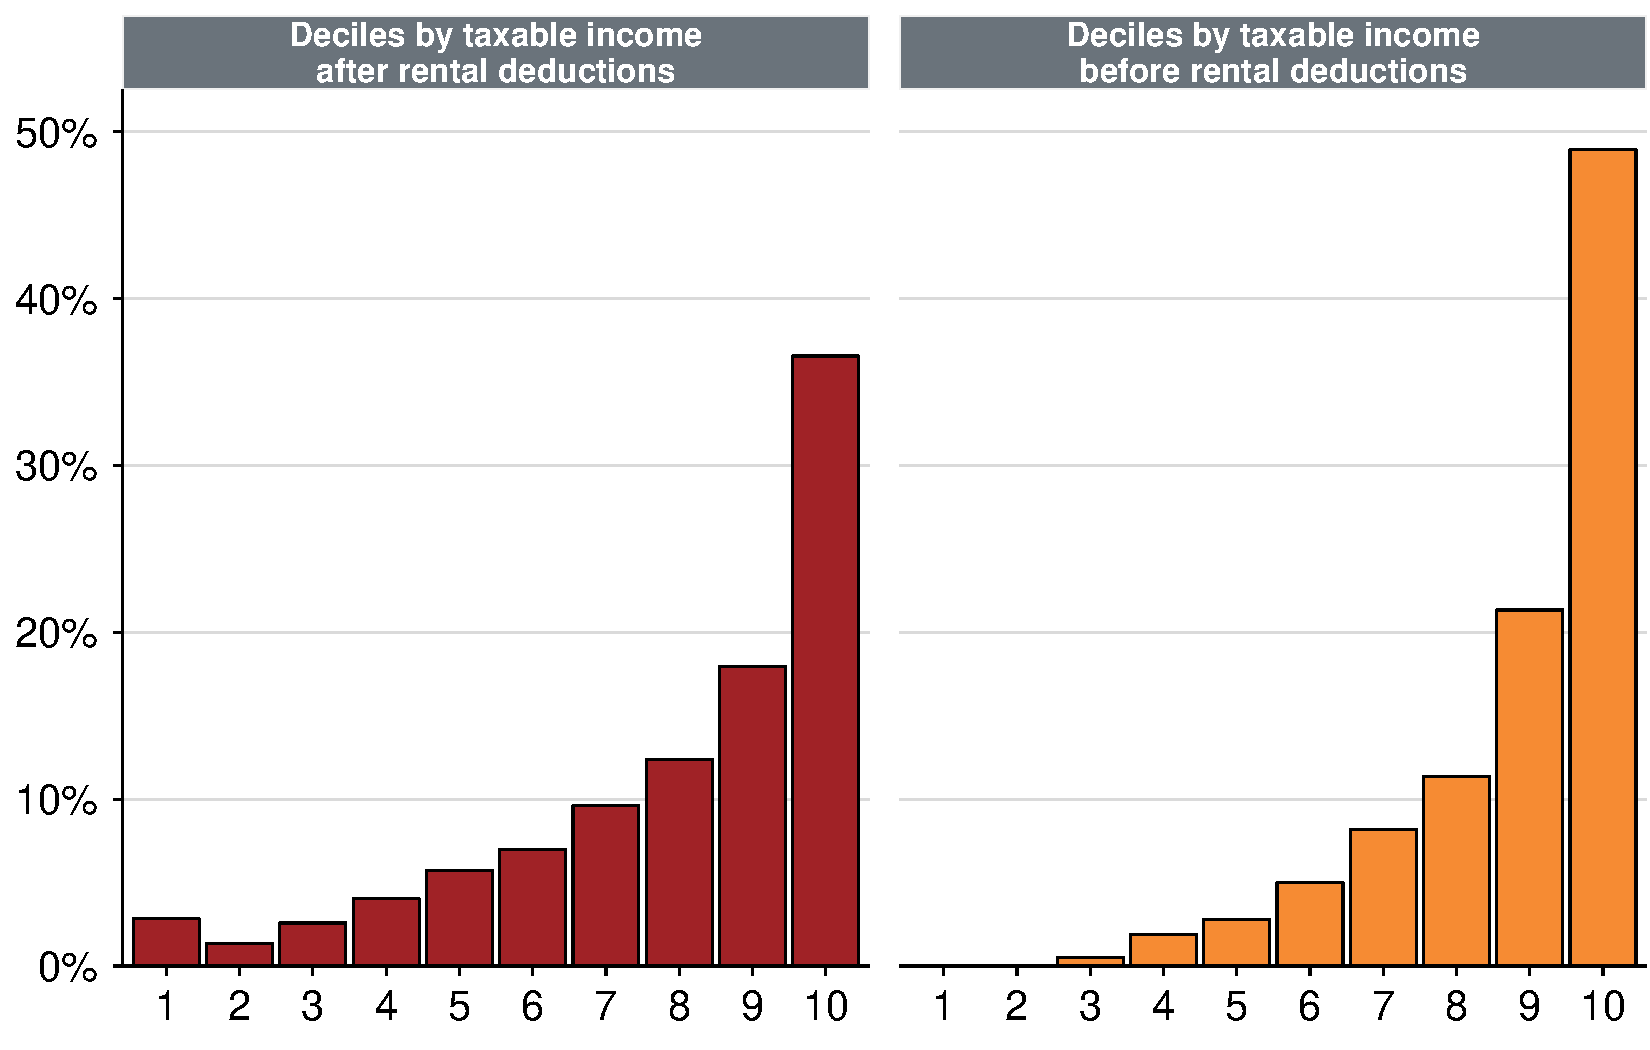
\includegraphics[width=\columnwidth]{figure/Effect_of_Deductions-1}
\notes{Taxable income before rental deductions means $\text{Taxable Income} - \min(\text{Net rental profit}, 0)$. Income tax includes medicare levy, medicare thresholds, but not other tax benefits (\emph{e.g.}~the seniors and pensioners tax offset (SAPTO))}

\source{\gao\ \textcite{ATO2013i}}
\end{figure}

\begin{knitrout}
\definecolor{shadecolor}{rgb}{0.969, 0.969, 0.969}\color{fgcolor}\begin{kframe}


{\ttfamily\noindent\bfseries\color{errorcolor}{\#\# Error in rbind(benefits\_by\_taxable\_income\_before\_deductions, benefits\_by\_taxable\_income): object 'benefits\_by\_taxable\_income\_before\_deductions' not found}}\end{kframe}
\end{knitrout}
% \begin{figure}
% \Caption{Negative gearing benefits mostly benefits those on high incomes, and the difference is especially stark when incomes are measured before subtracting rental interest deductions}{Average amount by which income tax was reduced due to negative gearing (2012-13)}  {fig:Effect_of_Deductions_amount}
% 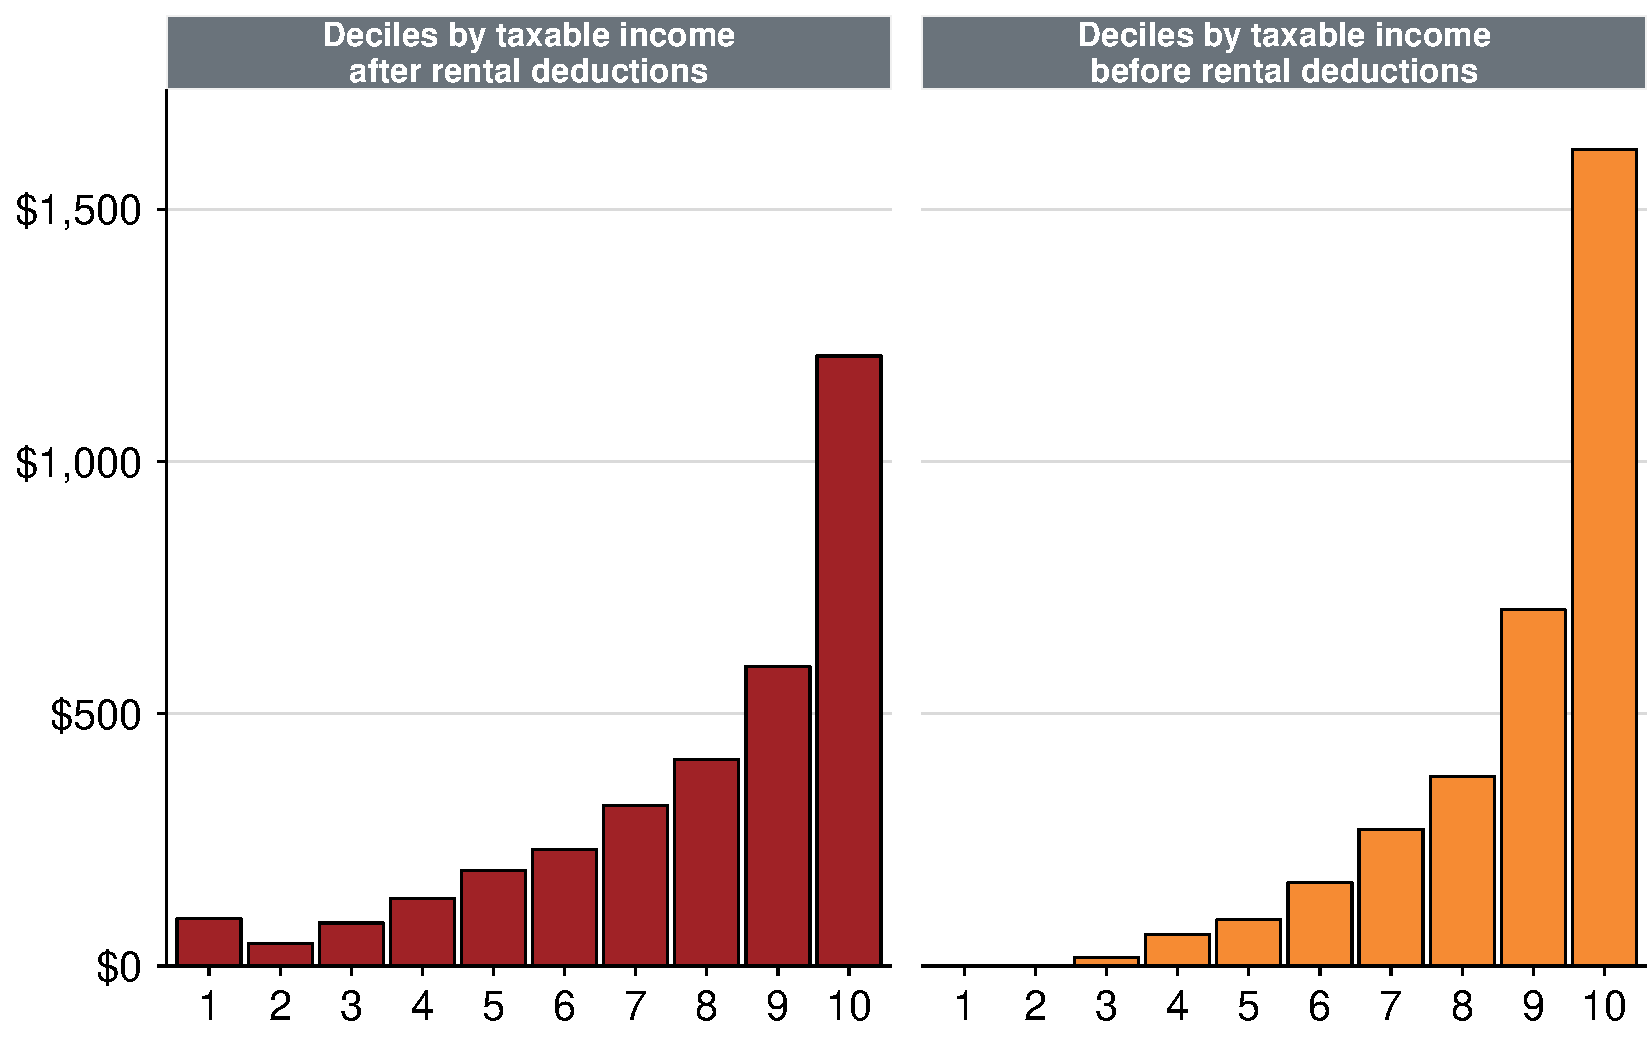
\includegraphics[width=\columnwidth]{figure/Effect_of_Deductions_amount-1}
% \notes{Income tax includes medicare levy,  medicare thresholds, but not other tax benefits (\emph{e.g.}~the seniors and pensioners tax offset (SAPTO))}
% 
% \source{\gao\ \textcite{ATO2013i}}
% \end{figure}

\subsection{Limiting negative gearing should not push up rents}
Concerns persist that limiting negative gearing will reduce the supply of rental properties and push up rents. Some of this seems to reflect folk memory from when the Hawke Government temporarily abolished negative gearing in the 1980s. Rents rose rapidly in Sydney and Perth. But adjusted for inflation, rents were stable in Melbourne and fell in Adelaide and Brisbane (\Vref{fig:Capital_city_rents}). In Sydney and Perth population growth and insufficient new housing, not tax policy, contributed to the rent rise.\footcite[pp.~47-48]{Daley2013}



\begin{knitrout}
\definecolor{shadecolor}{rgb}{0.969, 0.969, 0.969}\color{fgcolor}\begin{kframe}


{\ttfamily\noindent\bfseries\color{errorcolor}{\#\# Error: 'Capital\_city\_rents\_1980s.xlsx' does not exist in current working directory ('C:/Users/hparsonage/Negative\_gearing/Negative\_gearing').}}

{\ttfamily\noindent\bfseries\color{errorcolor}{\#\# Error in eval(expr, envir, enclos): object 'chart.dat' not found}}\end{kframe}
\end{knitrout}
\begin{figure}
\Caption{Negative gearing does not keep rents low. Only Perth experienced a considerable increase in rents without negative gearing. Adelaide and Brisbane actually experienced declines.}{Average rent prices (real compared with overall CPI), 1983 = 1. Grey band indicates the dates when negative gearing was not permitted}{fig:Capital_city_rents}
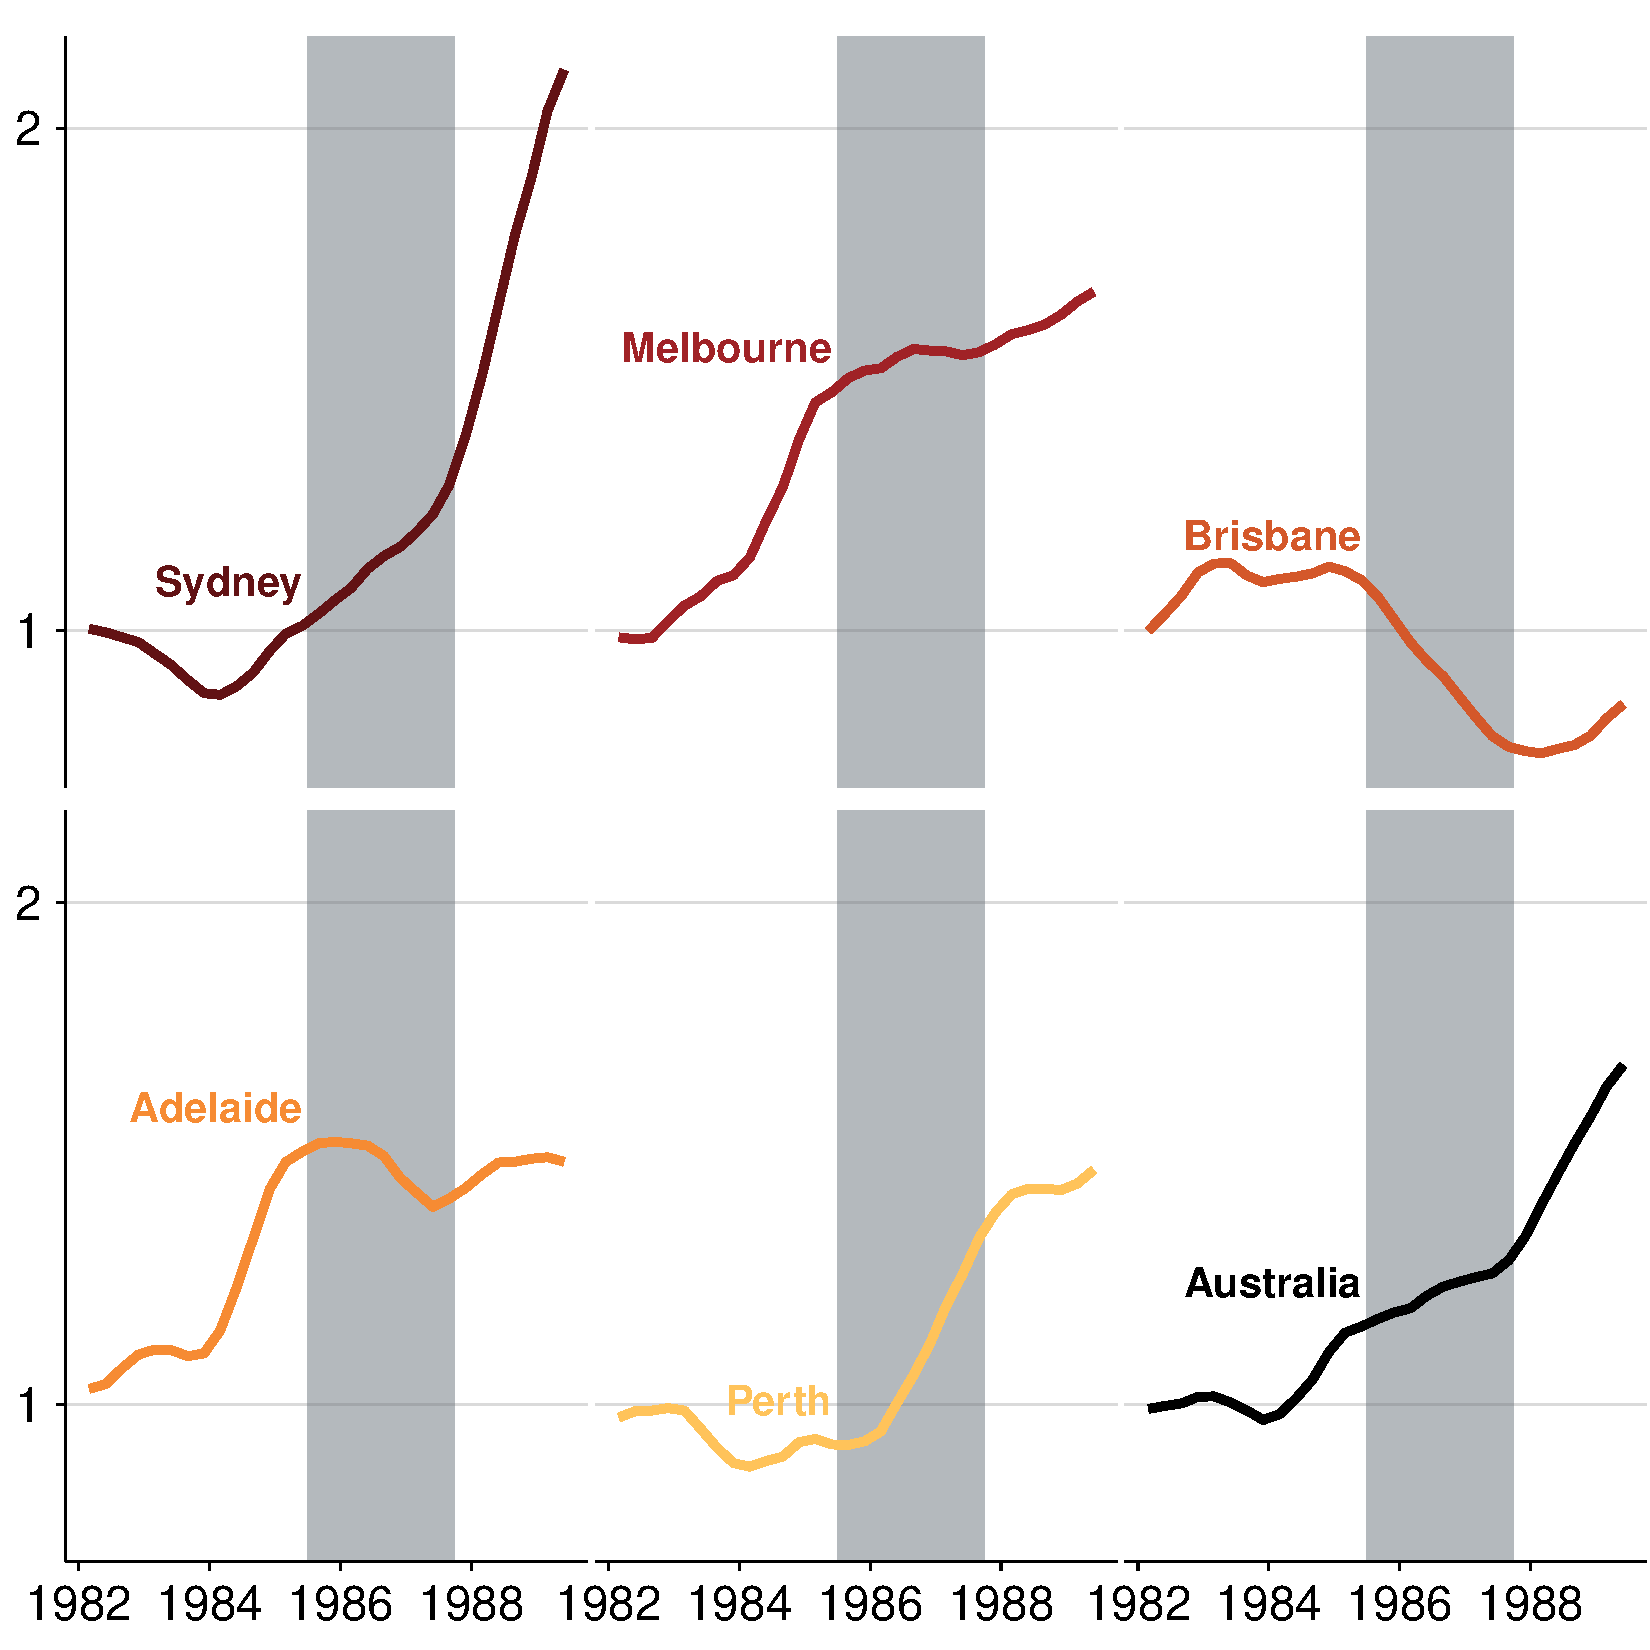
\includegraphics[width=\columnwidth]{figure/Capital_city_rents-1}
\source{ABS various years}
\end{figure}

Economic theory predicts that removing negative gearing should not change rents much. Every time an investor sells a property to a renter, there is one less rental property, and one less renter. There is no change to the balance between supply and demand of rental properties in the short term. 

It is also unlikely that removing negative gearing would affect the supply of new dwellings much over the medium term. Currently 93 per cent of all investment property lending is for existing dwellings.\footcite{ABS2015} Less investor demand would depress overall house prices and therefore returns to new construction.\footnote{The price transmission will be somewhat muted by the fact that the market for new housing, typically at the edge of cities, is somewhat detached from the market for established housing typically closer to the centre \textcite[See]{Kelly2011}.} But the main constraint on new housing is land release and zoning restrictions rather than the profitability of developments.\footcite[pp.84-90]{Kelly2013}

\section{Depreciation allowances also provide substantial tax advantages for investors}
Negative gearing and capital gains tax liabilities also interact to provide overly generous tax advantages to investors through depreciation allowances. 

Allowing capital works deductions for buildings and depreciation of fixtures and fittings is consistent with the principle that the costs of generating taxable income should be deductible.\footcite{Commission2004}  Property investors receive generous depreciation and capital allowances which they can write off in full against their taxable income. Capital works deductions can generally be claimed for construction costs and capital improvements at the rate of 2.5 per cent a year.\footcite{ATO2014b} The decline in value for other fixtures and fittings -- for example, window dressings or whitegoods -- can also be claimed as an expense.\footcite{ATO2014c}

When the asset is sold, the capital gain is based on a cost base calculated from the original purchase price, plus any improvements, less the depreciation claimed.\footcite[p.~21]{ATO2014d} This provides investors with a tax benefit: they write off the allowance at their marginal tax rate, but it is only clawed back at the discounted capital gains rate.\footnote{\textcite{RBA2014}. Most countries have more restricted depreciation allowances for investment housing. Others such as the UK and the Netherlands do not allow any depreciation writes offs. \textcite{Commission2004}}  In effect, investors receive a substantial tax windfall \Vref{box:Tax_advantage_from_capital_works_deductions}.  

\begin{smallbox}{Tax advantage from capital works deductions}{box:Tax_advantage_from_capital_works_deductions}
The property \$750,000 Hayley purchases was built in 1995. Her accountant estimates that the construction cost of the property for capital works deduction purposes is \$250,000, which includes the cost of the house, the pool and the recently constructed patio. 

Hayley claims capital works deductions of 2.5 per cent each year. She holds the property for ten years giving her deductions of \$56,000 over the period. If she remains in the top tax bracket, she receives capital works tax deductions of \$27,400 over the 10 years. 

When she sells the property for \$1 million, her capital gain is the difference between the selling price of the house and the cost base. If she has not made any further improvements to the property, the cost base will be the \$750,000 purchase price minus the \$56,000 in capital works deductions. Hayley's gross capital gain is \$194,000, she pays \$48,000 of this in tax. Because of the capital gains discount, only \$13,700 of the deductions she has claimed on capital works are clawed back through the tax on capital gains.

In effect, the owner nets a windfall for the amount of the capital works deductions claimed, multiplied by half of their marginal rate.
\end{smallbox}
Because of the interaction with the capital gains tax discount, Australia's treatment of depreciation appears to be more favourable than the treatment in other countries.\footcite{RBA2014}

\section{Options for reform}
The favourable tax treatment of investments -- particularly the interaction of the negative gearing arrangements with the capital gains tax discount -- have promoted speculative investment in housing while also costing the budget bottom line. 

Reducing the capital gains tax discount is the most direct way to reduce the incentive for inefficient investment activity. At the same time, negative gearing should be restricted so that losses from investments cannot be deducted against wage and salary income. The tax treatment of depreciation should also be changed to remove the preferential tax advantages generated by the asymmetric treatment of gains and losses. 

Reforms to capital gains tax or eligibility for negative gearing should apply to all types of assets, not just rental properties, so that the tax system does not encourage investors to favour one type of investment over another.  \footcite[p.~133]{Commission2004}

\subsection{Reducing the capital gains tax discount}
Reducing the capital gains tax discount would make the investment tax regime more efficient and fair. 

There are good arguments to abolish the capital gains tax discount altogether. It is not obvious why returns from investment should be taxed less that returns to working. And the differential tax rates create incentives for people to convert labour into capital income. 

But the arguments advanced for maintaining concessional treatment of gains sound a word of caution. While there is no compelling evidence that changes in tax rates materially change savings and investment behaviour, most studies examining these issues look at changes in behaviour in response to relatively modest changes in tax rates. Eliminating the capital gains tax discount would at least double the effective tax rate paid on capital returns. No OECD country taxes capital gains at full marginal tax rates in all circumstances. 

A more cautious approach would be to reduce the discount. Reducing the discount to 30 per cent, could raise around \$4 billion. Because this estimate does not include the effect on asset prices and investor behaviour, actual revenue raised is likely to be somewhat lower. On the other hand, these revenues should rise over time as capital losses built up from the GFC pass through the system.\footnote{CGT revenues are yet to recover following the GFC. Receipts were 0.46 per cent of GDP in 2012-13, down from a peak of 1.56 per cent of GDP in 2007-08. Even as asset prices have improved, capital losses carried forward have limited taxable gains. \textcite{Stewart2015}; \textcite{PBO2014}. }

This proposal would also be strongly progressive. Taxing capital gains in the same way as income would have very little effect on the tax burden for those in the bottom 20 per cent of the income distribution that earn little in the way of gains, as shown in \Vref{fig:Nearly_eighty_per_cent_of_capital_gains_are_earned_by_those_}. 

Reducing the discount will not entirely eliminate the distortions in investment decisions from the asymmetric treatment of gains and losses, but it will go some way towards it particularly if done in conjunction with limiting the deductibility of losses (see below). 

A partial removal of the discount, particularly if introduced slowly over time (\Vref{sec:transitional_arrangements}), will allow monitoring of the effects on investment markets. 

\subsection{Limiting negative gearing}
There is also a strong case for limiting the tax deductibility of losses. Quarantining losses so they cannot be written off against wage and salary income would limit the current distortions. 

While the deductibility of investment expenses including income expenses, has a strong grounding, there is no reason that these expenses should be deducted against wage and salary income.

This proposal would raise additional tax revenue in the short term, although the estimates are sensitive to changes in the housing market and the holding periods for assets. Applying the average marginal tax rate to the average annual rental losses of \$10.4 billion would yield \$4.2 billion in additional tax revenue in the short-term. 

Over the medium term, rental losses will start to be written off against income from capital gains. Assuming no change in investor behaviour, the additional tax revenue net of lower capital gains tax revenue would revert to around its average level of \$1.5 billion a year. 

But behavioural change is likely. Investments that make income losses are less attractive when the tax benefits can only be realised on sale. Much of the appeal of negative gearing lies in the scope to reduce annual taxes on wage income (\Vref{sec:negative_gearing_provides}). Removing the tax incentive for leveraged investment should result in investors shifting toward income producing assets and therefore an overall increase in income tax collections.  

\subsection{Matched discount and claimable losses}
An alternative proposal put forward in the Henry review was to discount rental losses by the same amount as the capital gains tax discount.\footcite[pp.~70,72]{Treasury2010}  In other words, only 50 per cent of expenses (including interest) associated with investments would be allowed as deduction against wage and salary income.  This proposal could also raise an additional \$2 billion each year for the budget. 

By restoring the symmetry in the treatment of gains and losses, investors would have less incentive to `chase' capital gains rather than recurrent income.\footcite[p.~418]{Treasury2010}

\subsection{Improve tax treatment of depreciation}
If capital gains tax discounts remain in place, then the taxation of depreciation allowances should also be reformed. When an asset is sold and the sale price is more than the purchase price, depreciation should not be deducted from the cost base for the purposes of calculating the capital gain. Instead, the tax deduction already received for depreciation should be refunded in full.\footnote{This is a variant of a proposal recommended by Rider and Stewart in their submission to the Productivity Commission Review of First Home Ownership. \textcite{Rider2004}}

This would remove the current tax advantage for depreciation because discounted capital gains tax arrangements only recoup half of the depreciation deductions claimed (section 1.4).  Each year around \$2 billion dollars is claimed in capital works allowances. If the depreciation previously claimed on these works were fully refunded, rather than recouped at the 50 per cent capital gain tax rate, this would raise up to an additional \$1 billion each year.\footnote{This estimate only includes building and capital works deductions and not depreciation for fixtures and fittings which are not reported separately by the ATO.  It does not include estimates of any behavioural change. It also assumes that investors are in the same tax bracket when the asset is sold as when the depreciation deductions are claimed. Because of the incentives to realise assets when tax rates are low this is an upper end estimate}

Investors would continue to receive the generous tax deferral advantages of the current depreciation regime.\footnote{Arguably current depreciation allowances are higher than the real economic depreciation of fixtures and fittings. Investors have an incentive to claim the maximum allowances. See \textcite[pp.~130-131]{Commission2004}.}

\section{Transitional arrangements}\label{sec:transitional_arrangements}
Whether governments choose to reform capital gains tax or negative gearing arrangements, changes should be phased-in to minimise sudden shifts in asset markets that are prone to over-shooting. Phase-in also provides investors with time to reorganise their affairs to adjust to the new regime.

Immediate reform to the current capital gains discount or negative gearing regimes would encourage investors to sell before the new legislation came into force. This could be moderated by phasing in the changes over a number of years. For example, under a ten year phase-in, the capital gains discount could be reduced to 45 per cent in the first year, and then reduced by five percentage points each year until all capital gains are taxed at the full marginal rate. Similarly, changes to Negative gearing could be phased in. For example, taxpayers might be allowed to claim only 90 per cent of their losses against wage and salary income in the first year (the remainder capitalised against any future capital gain), and the ten percentage points less each year until no losses are claimed against wage and salary income.

A less preferable alternative would be to grandfather existing arrangements. Those who purchased assets before capital gains tax reform was implemented could still claim the capital gains tax discount, even if they sell the assets several years afterwards. Similarly, those who purchased assets before negative gearing reform, could continue to claim all of their losses against their wage and salary income until the asset was sold.

Grandfathering causes a number of problems: it adds to complexity, reduces liquidity, and treats investors -- particularly younger investors -- unfairly.

Applying different tax treatments to investments depending on when they were acquired adds to the complexity of the tax system. Because investors can hold assets for decades, these dual tax arrangements are long-lived.  For example, the decision to grandfather the capital gains tax free status for assets purchased before 1986 still contributes to the complexity of our capital gains tax regime, 29 years later.\footcite[p.~75]{Treasury2010} 

Grandfathering arrangements reduce liquidity because investors have substantial incentives to retain whichever assets they purchased before the reform was implemented. They will be reluctant to buy and sell because the after tax returns on the assets bought earlier will be higher. Such a drag on liquidity is economically inefficient because it encourages investors to hold assets even when others could extract a higher return from them. This is a particular concern with negative gearing where a landlord may continue to hold a property because it generates ongoing deductible losses, even though an alternative owner might profitably develop the property. Grandfathering also exacerbates intergenerational inequality.\footcite{Daley2014}  Those who own assets before the reforms -- more likely those who are older -- earn higher after tax returns than those who start to build wealth later on.\footcite[p.~14]{Daley2014} 

Grandfathering arrangements are often driven by the principle of retrospectivity. However, this principle is often misunderstood. Concerns arise if a person acts as they would not otherwise because of a government policy, and then that policy changes to their detriment. Legitimate expectations, for which government is responsible, are defeated. But the concerns are much weaker if the person would have acted in the same way even if the new policy had been in place.

This is particularly relevant if the capital gains tax regime is changed for all asset classes. The after tax return for all asset classes (other than bank deposits) would be affected simultaneously. It is not obvious that investors would have saved less if there had been no capital gains tax discount.\footnote{Tax incentives for savings have greater effect on the choice of investment vehicle rather than the overall savings rate (see section 5.2 for discussion).} However, investors might have invested differently. In particular, they might well have invested less in property without the attraction of the negative gearing arrangements. 

Nor is the principle of retrospectivity absolute. Governments are entitled to change tax rates. If a person buys BHP Billiton shares, they cannot expect that the marginal tax rate then in force will still apply when they sell. No investor is entitled to a particular after-tax return in perpetuity.

Grandfathering (rather than a phase-in) may help existing owners less than they think. Abolishing the capital gains discount or restricting claims for losses on investments would reduce the after-tax returns for new purchasers. This would reduce the price they are prepared to pay existing owners.\footnote{This assumes that demand is dominated by potential new owners who would be affected by the new tax arrangements. An alternative approach would identify the "marginal investor", and expect a change in price only if they were affected by the new tax regime. In reality, demand is inevitably a combination of potential investors, subject to a variety of tax regimes, and the effect on price will depend on the extent of the tax change, and the proportion of potential investors affected.} A phase-in -- which treated old and new owners alike -- would have less immediate price impacts.

If grandfathering is nevertheless adopted, complexity in the long-term might be reduced by a sunset clause. This would provide that the new tax arrangements would apply to assets bought before the reforms if they were sold more than (say) fifteen years after the reform. This would provide existing owners ample time to reorganise, few investment assets are held for this long, and it would reduce complexity in the long-term.

The most powerful argument for grandfathering is political economy: those who benefit from the current arrangements are likely to be the most vociferous opponents of reform. It may be better to grandfather existing arrangements -- thereby muting opposition -- than to abandon worthwhile reform altogether.  
Nevertheless, given the competing considerations, phase-in would be a better transition. There would be less complexity, less immediate impact on prices, and younger investors would be treated more fairly. Concerns about investor expectations are not particularly strong as the phase-in proposed would provide them with ample time to reorder their affairs.

\onecolumn
%% Costings data
\begin{knitrout}
\definecolor{shadecolor}{rgb}{0.969, 0.969, 0.969}\color{fgcolor}\begin{kframe}
\begin{alltt}
\hlstd{new.discount} \hlkwb{<-} \hlnum{0.30}
\hlstd{discount_only_to_negative_rent_income} \hlkwb{<-} \hlnum{TRUE}
\end{alltt}
\end{kframe}
\end{knitrout}


Under this proposal, in which the discount is only applied to negative rental income, income tax would rise from \$159.2~billion to \$161.8~billion.

\section{Daley (quarantining salary from losses), 30\%\ discount}
\subsection{Parameters}


\begin{knitrout}
\definecolor{shadecolor}{rgb}{0.969, 0.969, 0.969}\color{fgcolor}\begin{kframe}
\begin{verbatim}
## R version 3.2.0 (2015-04-16)
## Platform: x86_64-w64-mingw32/x64 (64-bit)
## Running under: Windows 7 x64 (build 7601) Service Pack 1
## 
## locale:
## [1] LC_COLLATE=English_Australia.1252  LC_CTYPE=English_Australia.1252   
## [3] LC_MONETARY=English_Australia.1252 LC_NUMERIC=C                      
## [5] LC_TIME=English_Australia.1252    
## 
## attached base packages:
## [1] grid      stats     graphics  grDevices utils     datasets  methods  
## [8] base     
## 
## other attached packages:
##  [1] proto_0.3-10                parallelRandomForest_4.6-10
##  [3] foreach_1.4.2               randomForest_4.6-10        
##  [5] zoo_1.7-11                  httr_0.6.1                 
##  [7] rsdmx_0.4-6                 readr_0.1.1                
##  [9] readxl_0.1.0                xtable_1.7-4               
## [11] grattan_0.2                 directlabels_2013.6.15     
## [13] quadprog_1.5-5              scales_0.2.4               
## [15] ggplot2_1.0.0               gridExtra_0.9.1            
## [17] devEMF_2.0                  car_2.0-24                 
## [19] magrittr_1.5                tidyr_0.2.0                
## [21] dplyr_0.4.2                 data.table_1.9.4           
## [23] knitr_1.10.9               
## 
## loaded via a namespace (and not attached):
##  [1] reshape2_1.4.1   splines_3.2.0    lattice_0.20-31  colorspace_1.2-4
##  [5] mgcv_1.8-6       chron_2.3-45     XML_3.98-1.1     nloptr_1.0.4    
##  [9] DBI_0.3.1        plyr_1.8.3       stringr_0.6.2    munsell_0.4.2   
## [13] gtable_0.1.2     codetools_0.2-11 evaluate_0.7     labeling_0.3    
## [17] SparseM_1.6      quantreg_5.05    pbkrtest_0.4-2   parallel_3.2.0  
## [21] highr_0.4        Rcpp_0.11.5      formatR_1.0      lme4_1.1-7      
## [25] digest_0.6.8     tools_3.2.0      bitops_1.0-6     lazyeval_0.1.10 
## [29] RCurl_1.95-4.5   MASS_7.3-40      Matrix_1.2-0     assertthat_0.1  
## [33] minqa_1.2.4      iterators_1.0.7  R6_2.0.1         nnet_7.3-9      
## [37] nlme_3.1-120
\end{verbatim}
\end{kframe}
\end{knitrout}
\twocolumn

\printbibliography
\end{document}
